The search for heavy photons with displaced vertices is centered on the idea that the experimental vertex resolution is Gaussian ($N\propto e^{-z^2/\sigma^2}$) and that heavy photons have a measurable lifetime with an exponential decay length ($N_{A^{\prime}}\propto e^{-z/\gamma c\tau}$). Therefore, beyond a certain distance $z$ from the target, there should be almost no background but still some $A^{\prime}$ signal. The goal of this analysis to search for the heavy photon signal in a region of little to no background. We choose two-cluster events with an energy sum greater than 80$\%$ of the beam energy having tracks that match to ECal clusters. We reconstruct the vertex position between the pairs of tracks at the point of closest approach and measure the invariant mass of the pair from the momenta. We select an unbiased sample of events with low background by choosing a downstream position $zCut$ at which we can reject backgrounds and search for signal events.\\

\subsection{General event selection}
The event selection for the vertex analysis was optimized using a blinded data analysis such that the cuts were tuned on 10$\%$ of the data. The events relevant to the vertex analysis were triggered using the pairs-1 HPS trigger cuts. This loose trigger selects events that have a cluster each in the top and bottom of the ECal. The measured sum of the energy of the two reconstructed particles is chosen to greater than 80$\%$ of the beam energy to optimally search for $A^{\prime}$ events and reject Bethe-Heitler background. Tracks are reconstructed using various methods and a Generalized Broken Lines (GBL) track re-fit is performed using a minimum of five hits in a track. The closest approach of an $e^+e^-$ track pair is used to construct the vertex using an unconstrained vertex fit. The vertex $\chi^2$ quality of a beam spot constrained fit to the $e^+e^-$ pair was used to determine how well the momentum of the pair projects back to the beam spot position at the target.\\  
\indent The SVT tracks are projected to the ECal and matched to clusters based on position as a function of momentum. The match quality is measured in standard deviations, $n\sigma$, of the position difference for a given momentum. The ECal has better timing resolution than the SVT. The time difference between two clusters can be used to eliminate accidental coincidences and to study them. \\
\indent There are a few cuts that originate specifically from studies of high $z$ background events and physics processes which include cuts on the positron track's distance of closest approach in the $XZ$ plane to the target (DOCA), the $e^+e^-$ asymmetry, and the number of hits shared between tracks. 

\subsubsection{Vertex constraints}

The vertex search uses the unconstrained vertex fit to determine the $z$ vertex position of the $e^+e^-$ pair. The unconstrained fit uses only the distance of closest approach between the two tracks. We used the quality of the beam spot constrained fit, which considers both the point of closest approach between the two tracks and the momentum projection back to the beam spot position at the target, only as a data quality cut. For genuine $A^{\prime}$ displaced vertices, the $z$ vertex position is relatively unchanged when using a beam spot constrained versus an unconstrained vertex fit. An incorrect beam spot position can systematically pull a measured vertex position. Background events from prompt vertices that are pushed to large $z$ through measurement error or scatters can be arbitrarily biased in the $z$ vertex position by using the beam spot constrained fit. For these reasons, the unconstrained fit is used to determine $z$.\\

\section{Datasets}
We took 1.7~days (1166~nb$^{-1}$) of data with a 1.056~GeV beam with the SVT at the nominal position where Layer 1 is at $\pm$0.5~mm from the beam. We took an additional 0.47~days (362.7~nb$^{-1}$), prior to moving the SVT to the nominal position, with the SVT Layer 1 at $\pm$1.5~mm from the beam. A large portion of the data taken with the first layer of the SVT at $\pm$1.5~mm was unusable due to an incorrect timing latency in the SVT DAQ and is excluded from this analysis. We divided the data into six data sets as shown in Table~\ref{tab:datasets}. The data sets are determined by the first hit layer of the $e^+e^-$ tracks that make up the vertex. Each data set is exclusive of the other data sets. Events were excluded where the reconstructed track passed through the active region of the sensor and had no hit. 

\begin{table}[htb]
\caption{Vertexing Data sets}
\label{tab:datasets}
\centering
\begin{tabular}{lllr}
\toprule
%\multicolumn{2}{c}{Name} \\
%\cmidrule(r){1-2}
Data sets &First hit of track & SVT position & events \\
\midrule
L1L1 & Both tracks layer 1 & 0.5~mm & 13,697,082\\
L1L2 & One track layer 1 & 0.5~mm & 302,103\\
L2L2 & Both tracks layer 2 & 0.5~mm & 4,876\\
L1L1 & Both tracks layer 1 & 1.5~mm & 1,635,172\\
L1L2 & One track layer 1 & 1.5~mm & 1,005,668\\
L2L2 & Both tracks layer 2 & 1.5~mm & 233,388\\
\bottomrule
\end{tabular}
\end{table}
The backgrounds, statistics, and efficiencies are different for each dataset, and therefore require separate analyses before combining the limits of the final results of each.

\section{$A^{\prime}$ signal in the displaced vertex search}
We must select a downstream region for which to look for a heavy photon having virtually no background. Therefore, we choose a $zCut$ which is a downstream $z$ vertex position beyond which there should be fewer than 0.5~background event/bin. We arbitrarily choose our maximum $z$ value, $zMax$, to be at the first layer, although this can vary depending on the dataset. The $zCut$ varies as a function of mass and can be ideally selected to minimize backgrounds whilst maximizing $A^{\prime}$ production. The number of events we can expect to reconstruct is 

\begin{equation}
\label{eq:signal}
S_{bin,zCut} = \left( \dfrac{N_{rad}}{N_{tot}}\right) N_{bin}\left(\dfrac{3\pi\epsilon^{2}}{2N_{eff}\alpha}\right)\left(\dfrac{m_{A'}}{\delta m_{A'}}\right)\epsilon_{bin}\int_{zCut}^{zMax}\dfrac{e^{-ztgt-z/\gamma c\tau}}{\gamma c \tau}\epsilon_{vtx}(z,m_{A'})dz
\end{equation}
where the heavy photon production at the target per mass bin is described by the first four terms.  $N_{rad}/N_{tot}$ is the fraction of radiative events (see Figure~\ref{fig:radFrac}) contained in the sample and is derived from Monte Carlo. $N_{bin}$ is the number of measured $e^+e^-$ pairs at a given mass. The third and fourth terms are explained in Equation~\eqref{eq:crossSection}. $\epsilon_{bin}$ is the fraction of signal we reconstruct within our selected mass bin window (we choose a mass window of $\pm1.4\sigma_m$ corresponding to an $\epsilon_{bin}$ of 0.838). The integral calculates the expected number of heavy photons we would reconstruct in the decay region from $zCut$ to $zMax$, where $ztgt$ is the target location. $\epsilon_{vtx}$ represents the efficiency of detecting $e^+e^-$ pairs from an $A^{\prime}$ of mass $m_{A'}$ that decayed at position $z$ from the target and is inclusive of the efficiencies of all other cuts used in the analysis. Based on Poisson statistics, the 90$\%$ confidence limit for a null result requires us to have an expected number of $A^{\prime}$ events to be greater than 2.3.\\
\indent In order to find the value of $zCut$, we slice the distribution of the reconstructed vertex position versus reconstructed mass in bins of mass. We fit the core of the vertex distribution with a Gaussian and fit the downstream tail of the distribution with an exponential. The fit for the full vertex distribution in a given mass bin is:

\begin{equation}
\label{eq:vtxFit}
\begin{split}
F(z < b) & =  Ae^{-\dfrac{(z-z_{mean})^2}{2\sigma^2}}\\
F(z > b) & =  Ae^{-\dfrac{b^2}{2\sigma^2}-\dfrac{z-z_{mean}-b}{l}}
\end{split}
\end{equation}
where $b$ defines the distance from the core of the Gaussian that the fit will be described by the exponential tail. The exponential tail, where $z>b$, is defined in terms of the parameter $l$. The $zCut$ is selected by integrating this function so that there remains 0.5 background events downstream. A fit to a mass slice from the L1L1 dataset is shown in Figure~\ref{fig:vtxFitPic}.

\begin{figure}[htb]
  \centering
      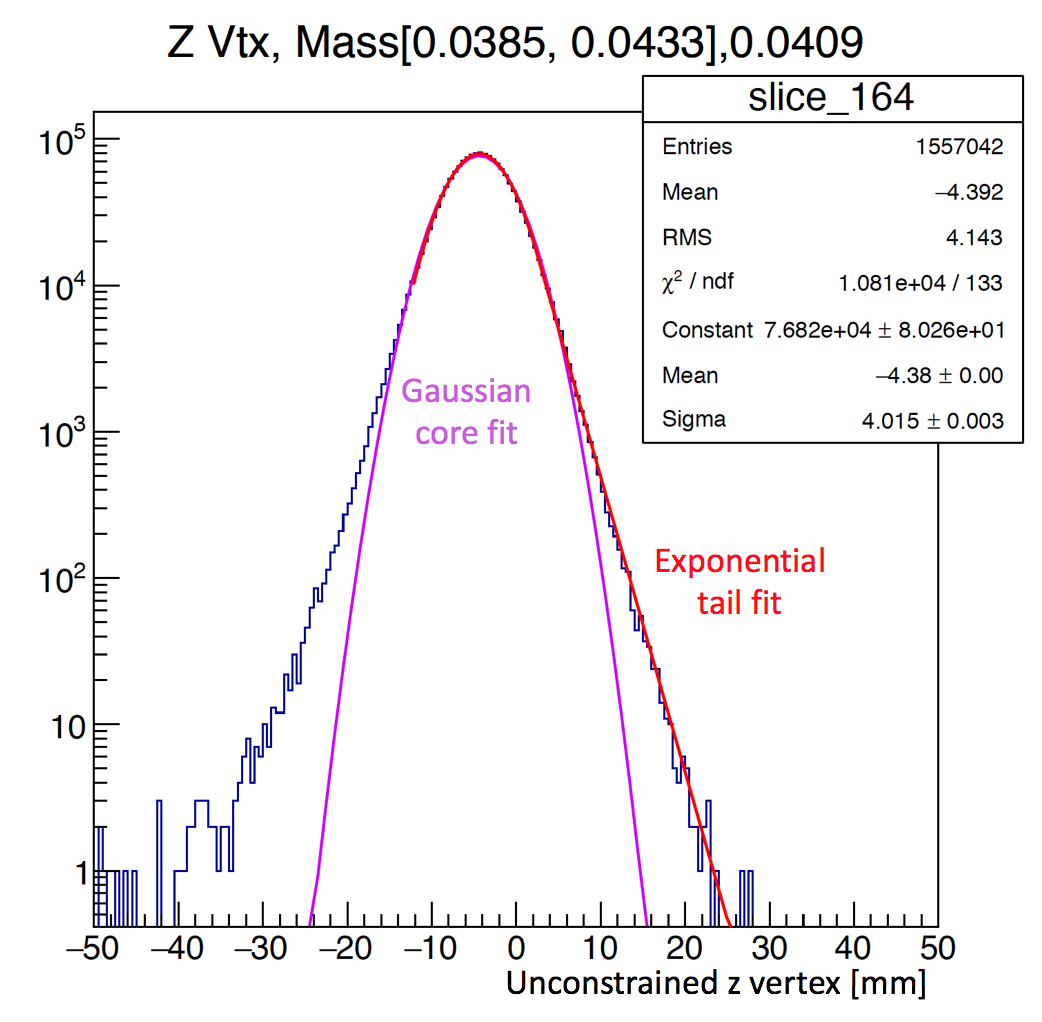
\includegraphics[width=0.6\textwidth]{pics/searching/vtxFit.png}
  \caption[Fit to vertex slice at a mass of 41~MeV]{The number of events versus $z$ vertex in the full L1L1 data set for a mass slice centered at 41~MeV. The fit functions are described by Equation~\eqref{eq:vtxFit} where the core of the distribution is fit with a Gaussian and the downstream tail is fit with an exponential. The $zCut$ is shown in green. The exponential fit is not shown in the statistics box.}
  \label{fig:vtxFitPic}
\end{figure} 


\subsection{Radiative Fraction}
Background events can be produced by QED trident processes and wide-angle bremsstrahlung (WAB). The trident processes can be separated into ``radiative" and ``Bethe-Heitler" diagrams. The heavy photon cross section is related to the radiative trident cross section. The $A^{\prime}$ production for a mass bin is

\begin{equation}
\label{eq:crossSection}
\dfrac{d\sigma(A'\rightarrow e+e-)}{d\sigma(\gamma*\rightarrow e+e-)} = \left(\dfrac{3\pi\epsilon^{2}}{2N_{eff}\alpha}\right)\left(\dfrac{m_{A'}}{\delta m_{A'}}\right)
\end{equation}
where $N_{eff}$, the number of available decay states, is one for the HPS experiment which explores a mass range in which the heavy photon can only decay to one Standard Model final state ($e^+e^-$). $\epsilon^{2}$ is the coupling factor between the heavy photon and the Standard Model while $\alpha$ is the fine structure constant. $\dfrac{m_{A'}}{\delta_{m_{A'}}}$ is the center of the mass bin divided by the bin width. \\%%among trident or all bg events??
\indent The fraction of radiative reactions among trident events in the HPS search region is the radiative fraction. Using MadGraph5 Monte Carlo to model the tridents and radiatives and the MadGraph4 Monte Carlo to model the wide angle bremsstrahlung (WAB) background, we found the radiative fraction to be approximately 9.5$\%$ for all masses (see Figure~\ref{fig:radFrac}). This fraction is defined as the ratio of radiative events to the background events (tritrig+WAB in Figure~\ref{fig:radFrac}) and is the same for both the 0.5~mm and 1.5~mm data sets.

\begin{figure}[htb]
  \centering
      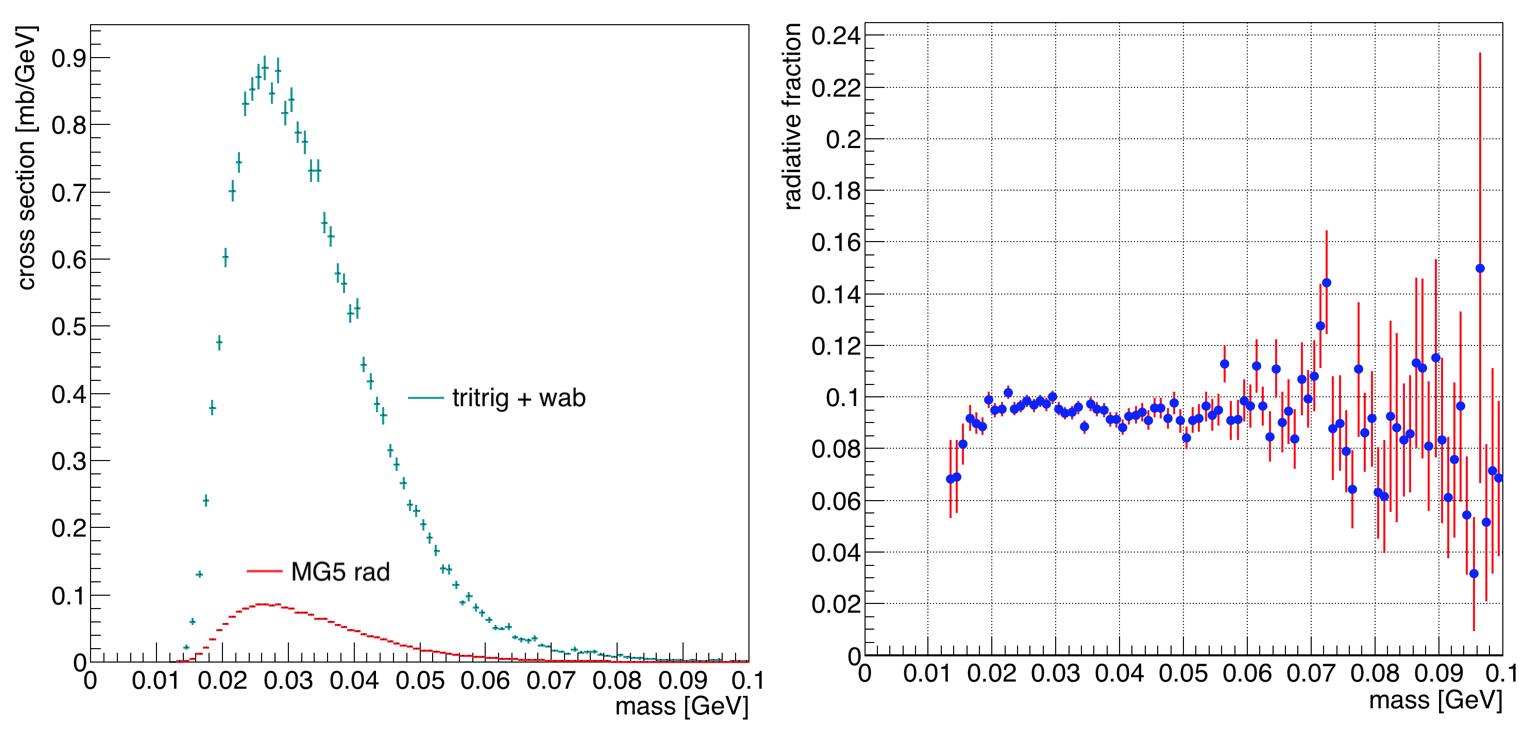
\includegraphics[width=0.9\textwidth]{pics/searching/radFrac.png}
  \caption[Radiative fraction from Monte Carlo]{The radiative fraction is the fraction of radiative events to all measured backgrounds. The plot on the left shows the background containing all trident diagrams and wide angle bremsstrahlung, inclusively, in blue and the radiatives in red. The ratio between these two curves is shown on the right with a roughly constant radiative fraction of 9.5$\%$.}
  \label{fig:radFrac}
\end{figure} 

\subsection{Vertex reconstruction efficiencies, $\epsilon_{vtx}$}
The integral described in Equation~\eqref{eq:signal} contains an $\epsilon_{vtx}$ parameter that describes the fraction of events we can reconstruct as a function of $z$ and includes both detector acceptances and inefficiencies. Using $A^{\prime}$ Monte Carlo, $\epsilon_{vtx}$ is measured from the ratio of the reconstructed heavy photon events to the generated heavy photons events as a function of both mass and $z$ vertex position. At each mass, the ratio of the reconstructed to generated heavy photon events is scaled such that for L1L1, the fitted ratio is 1 at that target position. The reconstruction efficiency at the target without scaling is shown in Figure~\ref{fig:rawEff}.

\begin{figure}[htb]
  \centering
      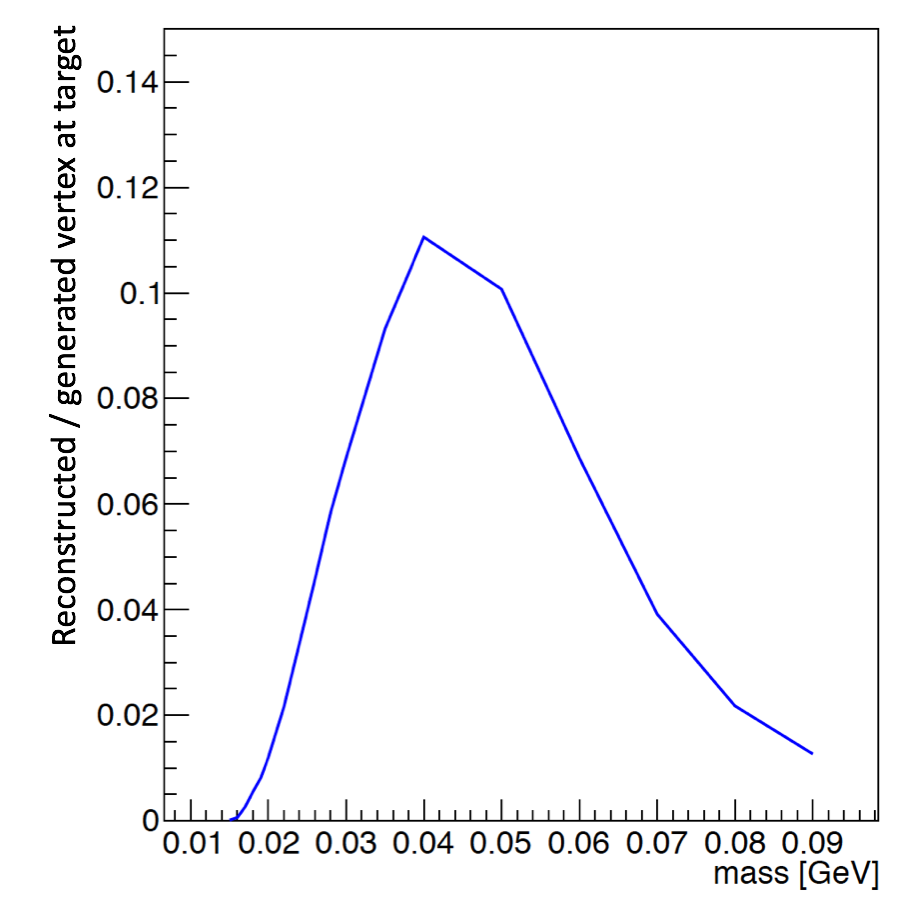
\includegraphics[width=0.5\textwidth]{pics/searching/rawEffL1L1.png}
  \caption[Reconstruction efficiency for heavy photons that decay at the target]{Reconstruction efficiency for heavy photon events with decay vertices at the target as a function of mass.}
  \label{fig:rawEff}
\end{figure} 

As shown in Figure~\ref{fig:rawEff}, the maximum efficiency in the HPS detector for events that decay promptly occurs around heavy photon masses between 40--50~MeV. This reconstruction efficiency at the target is normalized to 1, and the L1L2 and L2L2 data sets are scaled to ensure the same relative relationship between the three data sets. The reconstruction efficiencies for a 35~MeV heavy photon as a function of position are shown in Figure~\ref{fig:apEff}. 

\begin{figure}[htb]
  \centering
      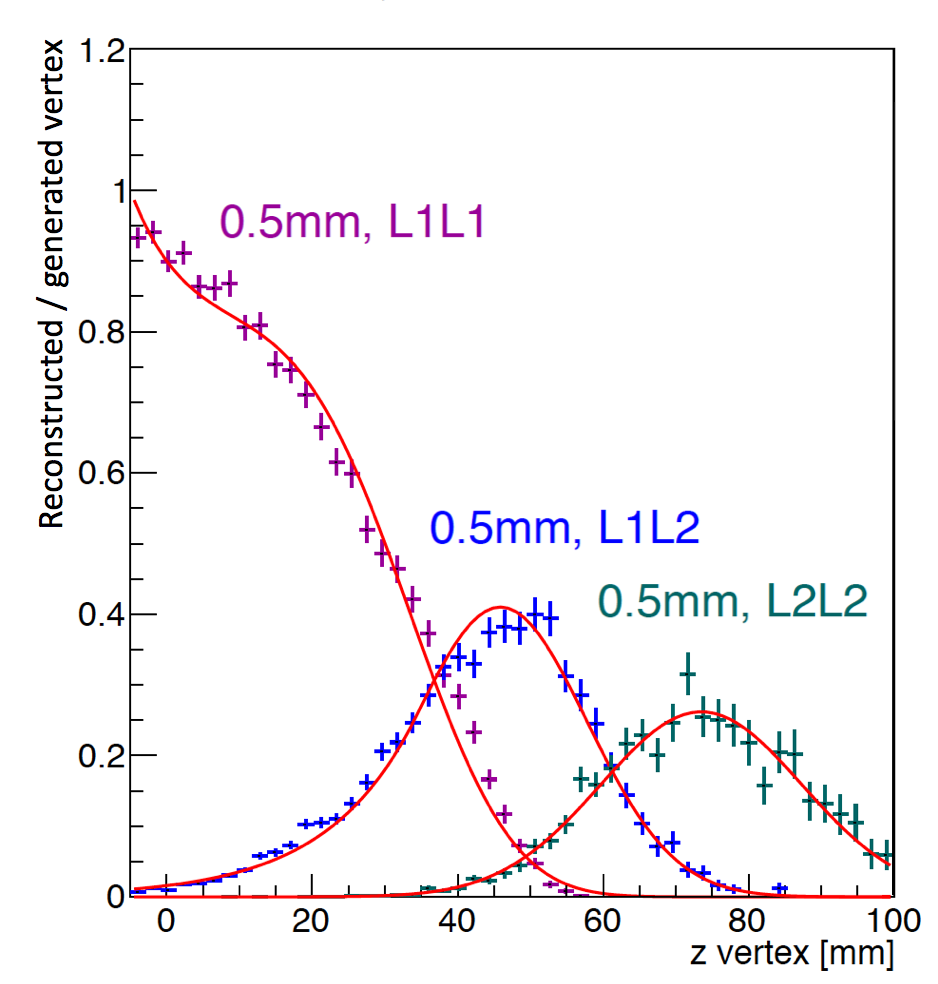
\includegraphics[width=0.65\textwidth]{pics/searching/reconstructedVtx.png}
  \caption[Fraction of reconstructed events of a 35~MeV $A^{\prime}$ as a function of decay vertex position]{Fraction of reconstructed events of a 35~MeV $A^{\prime}$ as a function of decay vertex position. The three datasets are mutually exclusive. Each data set is fit independently of the others and parameterized in terms of mass and $z$ vertex position. }
  \label{fig:apEff}
\end{figure} 
As all data sets are mutually exclusive, the total reconstruction efficiency for all $z$ vertex positions is the sum of the efficiencies for the individual datasets. These efficiencies are then integrated from different $zCut$ values to $zMax$ (set at the $z$ position of Layer 1, or 10~cm). The efficiency at each mass for each data set is fitted with a corresponding functional description that is parameterized in terms of mass and $z$ vertex position. The vertex reconstruction efficiency for the L1L1 data is 

\begin{equation}
\label{eq:promptfunction}
\epsilon_{vtx} = \exp(p_0+p_1z+p_2z^2+p_3z^3) 
\end{equation}
where all parameters are functions of mass. For the L1L2 data, the reconstruction efficiency improves farther downstream and is described by a Crystal Ball function as shown in Equation~\eqref{eq:cbfunction}.

\begin{equation}
\begin{split}
\label{eq:cbfunction}
\epsilon_{vtx}(t >= -| \alpha |) & = N e^{-0.5t^{2}}\\
\epsilon_{vtx}(t < -| \alpha |) & = N A(B-t)^{-n}\\
\textrm{where:}\\
\alpha & = 0.97\\
n & = 141.5\\
t & = \dfrac{z-z_{mean}}{\sigma}\\
A & = (\dfrac{n}{| \alpha |})^{n}e^{-0.5 |\alpha |^2}\\
B & = \dfrac{n}{| \alpha |}-|\alpha | \\
N & = \textrm{amplitude of the Gaussian}
\end{split}
\end{equation}
where the parameters $z_{mean}$, $\sigma$, and $N$ are obtained from fitting the distribution and are functions of mass. The L2L2 data set efficiency improves farther downstream than L1L2 and is best described by a Gaussian 

\begin{equation}
\label{eq:gausfunction}
\epsilon_{vtx} = Ne^{-0.5\dfrac{(z-z_{mean})^2}{\sigma^2}}
\end{equation}
The individual fit parameter values are shown in Appendix~\ref{appendix:vtxEff}.\\
\indent Once these relations are derived, we obtain a value for $\epsilon_{vtx}$ that is integrated over $z$ from the $zCut$ to $zMax$ to calculate a maximum fractional signal yield. The full integral is shown in Figure~\ref{fig:effIntegral} as the color $z$--axis and is a function of both the heavy photon mass and $zCut$.  

\begin{figure}[htb]
  \centering
      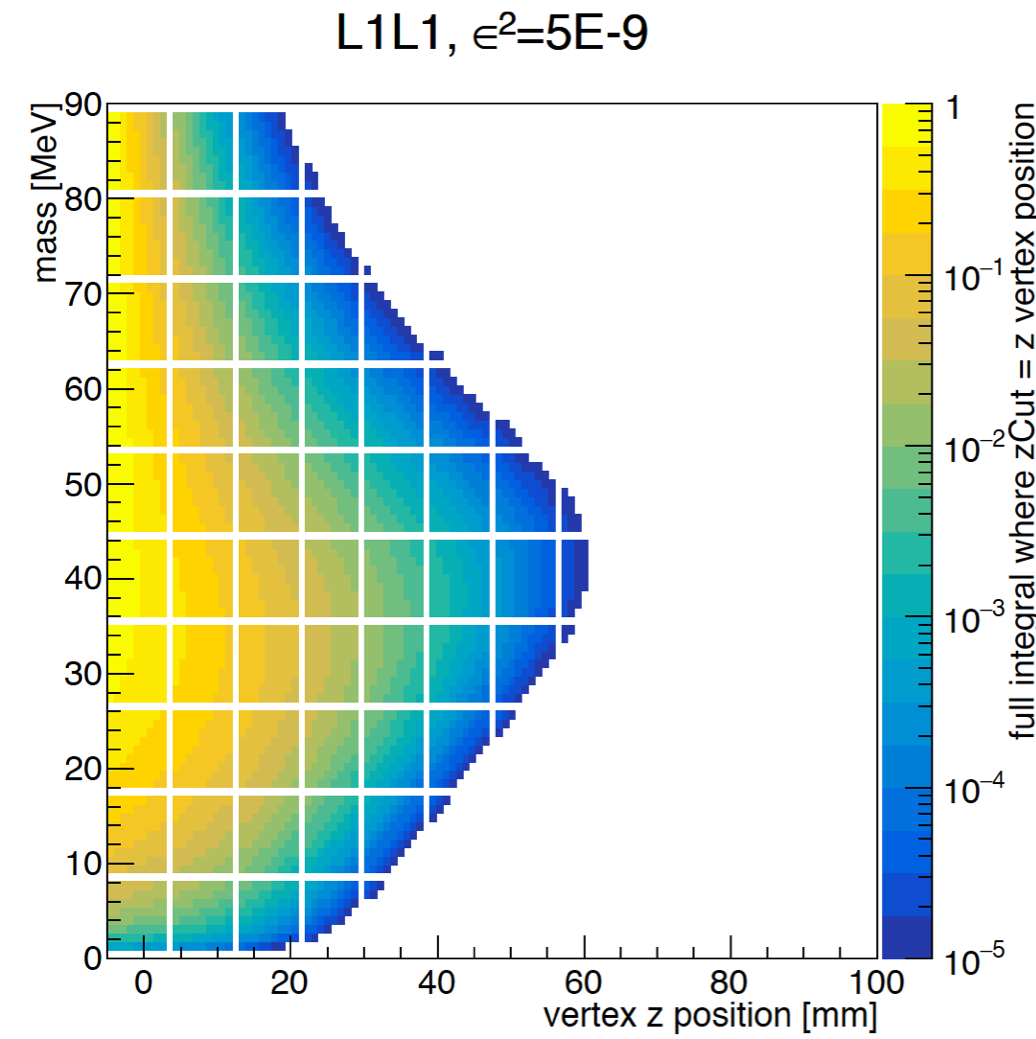
\includegraphics[width=0.65\textwidth]{pics/searching/integralEffL1L1.png}
  \caption[Integral as a function of mass and $zCut$ for L1L1]{The maximum fractional signal yield for the L1L1 0.5~mm data set as a function of $zCut$ and mass is shown. The coupling, $\epsilon^2$ is fixed here to $5E-9$ and $zMax$ is chosen to be 10~cm, corresponding to the $z$ position of the first SVT layer. }
  \label{fig:effIntegral}
\end{figure}

The full integral value yields some fractional number that, when multiplied by the expected heavy photon yield from the cross section, tells us how many heavy photons we can expect to reconstruct in the given decay vertex region. For the L1L1 data set, it is critical to set the zCut as low as possible in order to obtain the highest signal yield. Figure~\ref{fig:effIntegral} shows the value of the integral for $\epsilon^{2} = 5E-9$ as a function of mass and $zCut$. The same calculation for the L1L2 dataset is shown in Figure~\ref{fig:effIntegral12}.

\begin{figure}[htb]
  \centering
      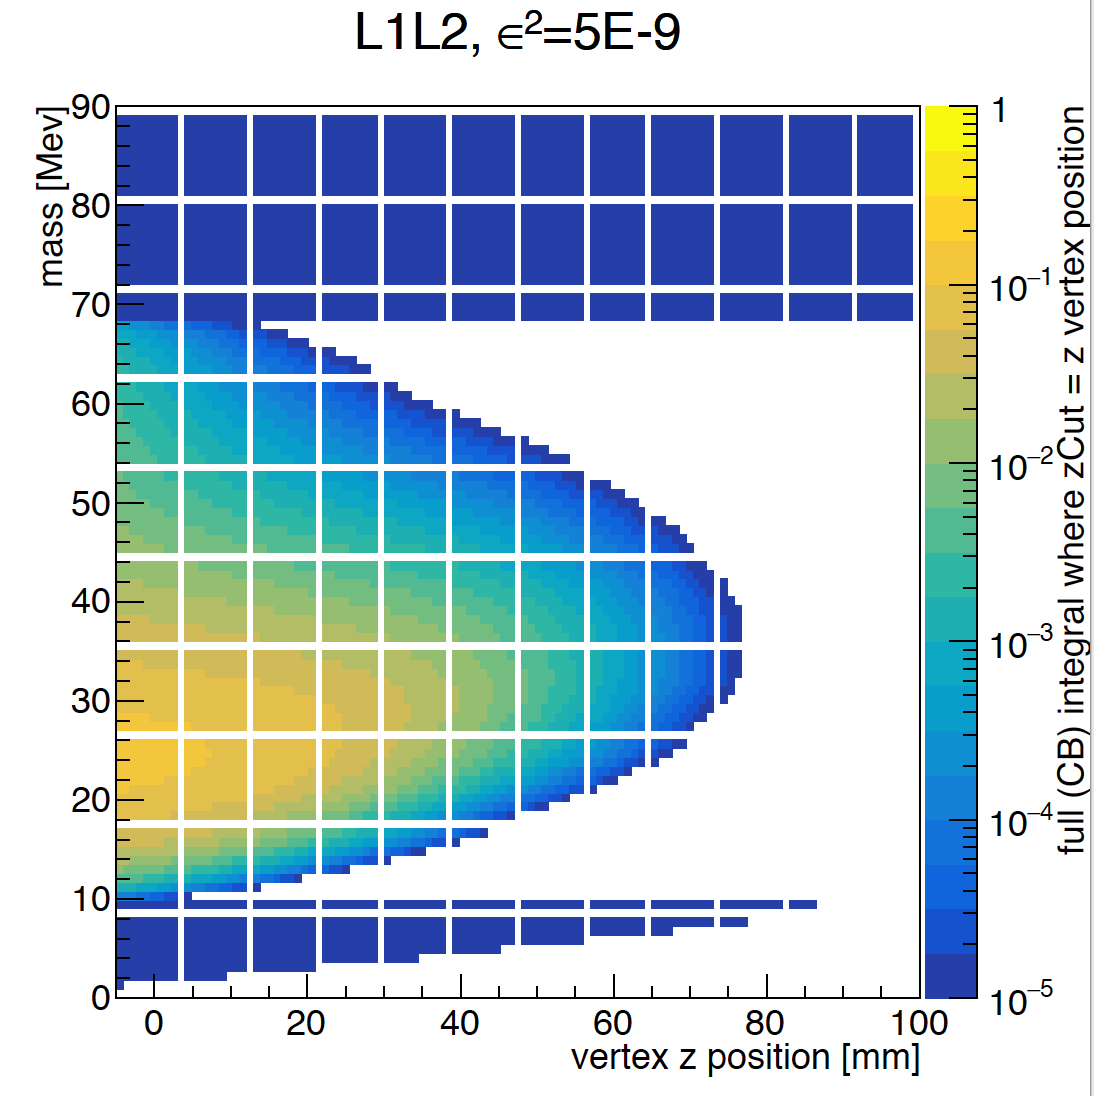
\includegraphics[width=0.65\textwidth]{pics/searching/integralEff12.png}
  \caption[Integral as a function of mass and $zCut$ for L1L2]{The maximum fractional signal yield for the L1L2 0.5~mm data set as a function of $zCut$ and mass for $\epsilon^2=5E-9$. $zMax$ is chosen to be 10~cm, corresponding to the $z$ position of the first SVT layer. }
  \label{fig:effIntegral12}
\end{figure}

The maximum fractional signal yield is significantly less for the L1L2 data set than for the L1L1 data set. The lifetime of the heavy photon in Figure~\ref{fig:effIntegral12} is not long enough to significantly benefit from the additional efficiency obtained at longer displaced $z$ vertex positions. The integrated efficiency for the L2L2 data is shown in Figure~\ref{fig:effIntegral22}.

\begin{figure}[htb]
  \centering
      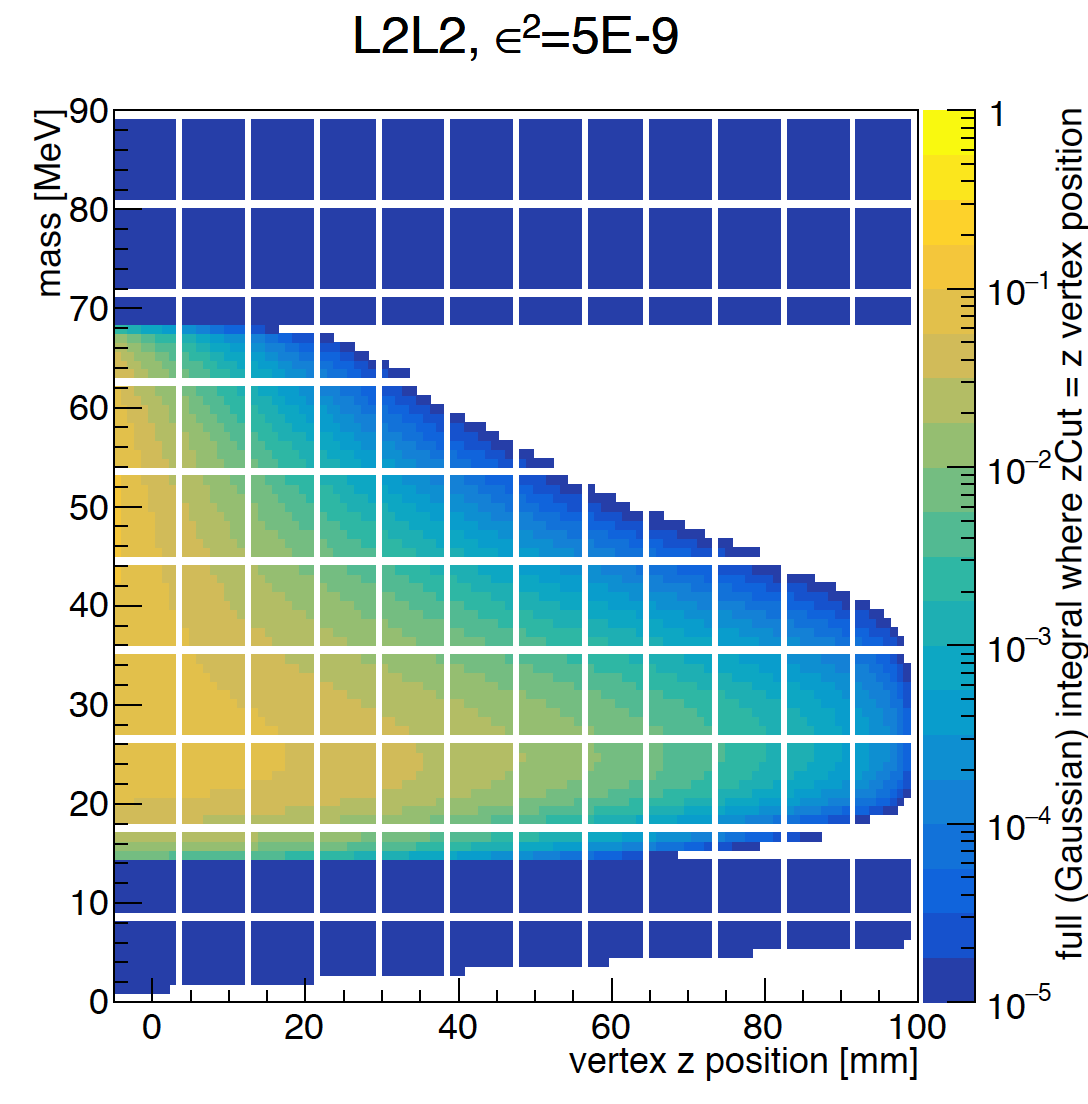
\includegraphics[width=0.65\textwidth]{pics/searching/integralEff22.png}
  \caption[Integral as a function of mass and $zCut$ for L2L2]{The integrated vertex efficiency, $\epsilon_{vtx}$, for the L2L2 0.5~mm data set as a function of the $zCut$ and mass is shown. The coupling, $\epsilon^2$ is fixed here to $5E-9$ and $zMax$ is chosen to be 10~cm, corresponding to the $z$ position of the first SVT layer. }
  \label{fig:effIntegral22}
\end{figure}

The fractional yield for the L2L2 data set is significantly less than  the L1L1 data set.  The L1L2 and L2L2 datasets are most useful for detecting lower mass $A^{\prime}$s with displaced $z$ vertex positions. 

\subsection{Mass resolution}
It was previously observed that the mass resolution in Monte Carlo deteriorated for displaced vertices. The problem arises due to the track parameters not being adjusted for the vertex position~\cite{billoir_fast_1992}. I used the following correction to the measured mass

\begin{equation}
\label{eq:massCorrection}
m_{corr} \textrm{ [GeV]}= m_{uc}\textrm{ [GeV]} - \dfrac{0.15\times 10^{-3}\times z_{vtx}\textrm{ [mm]}}{m_{uc}\textrm{ [GeV]}}\big(\dfrac{P_{x,e-}}{P_{e-}}-\dfrac{P_{x,e+}}{P_{e+}}\big)            
\end{equation}
where the unconstrained vertex mass is $m_{uc}$, the reconstructed $z$ vertex position downstream in mm is $z_{vtx}$, the horizontal momentum component is indicated by $P_x$ where the corresponding particle type is also indicated by the subscript, and the magnitude of the momentum is $P$. The effects of the correction to the reconstructed mass can be seen in Figure~\ref{fig:effectMCorr}.

\begin{figure}[htb]
  \centering
      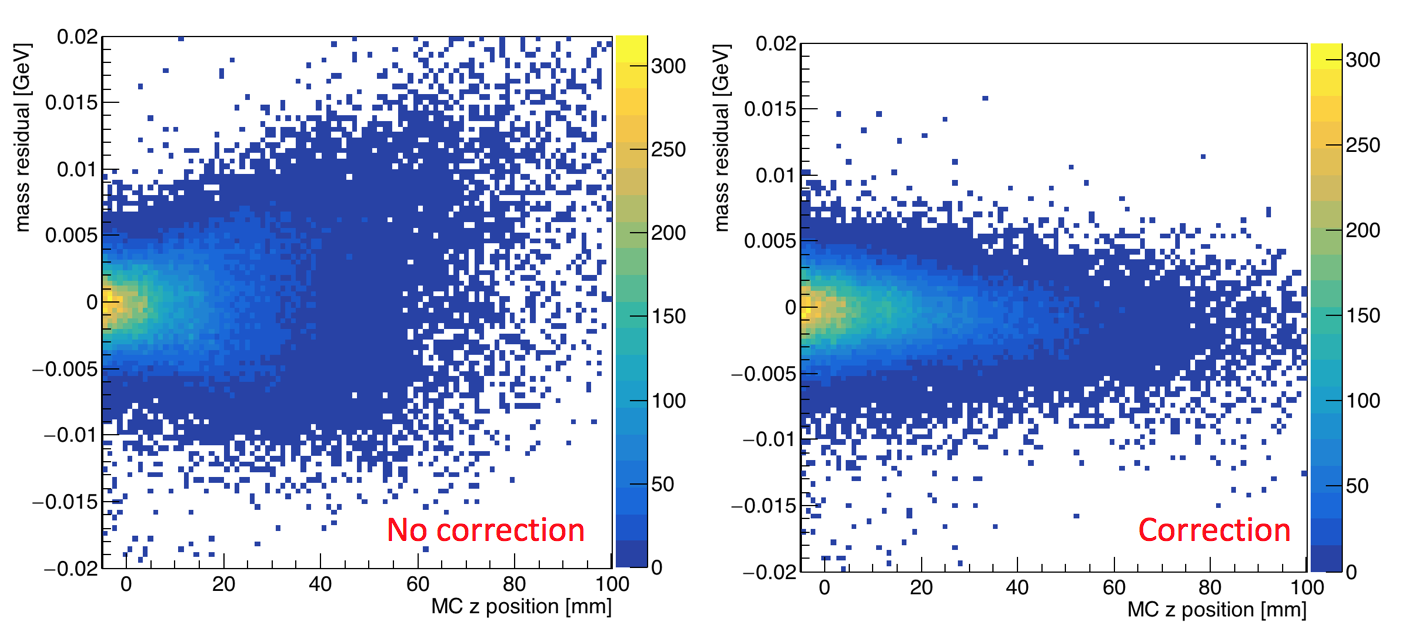
\includegraphics[width=0.9\textwidth]{pics/searching/massCorrection.png}
  \caption[Correction to the reconstructed mass for a 40~MeV $A^{\prime}$]{The mass residual of a reconstructed 40~MeV $A^{\prime}$ is shown as a function of vertex position in $z$. The uncorrected mass residual as given from the vertexer is shown on the left. The resolution deteriorates with the downstream $z$ position of the vertex. After the correction is applied, as shown on the right, the mass resolution is no longer vertex position dependent.}
  \label{fig:effectMCorr}
\end{figure} 

The mass resolution is determined from $A^{\prime}$ Monte Carlo and has been checked with the $e^-e^-$ mass resolution from M\o ller scattered electron pairs in data. By generating heavy photons at discrete masses, applying the cuts proposed in data, and fitting the $A^{\prime}$ mass peak residual with respect to the generated mass peak, the mass resolution can be measured as a function of mass. A fit to the generated 40~MeV heavy photon in Monte Carlo is shown in Figure~\ref{fig:ap40mev}.

\begin{figure}[htb]
  \centering
      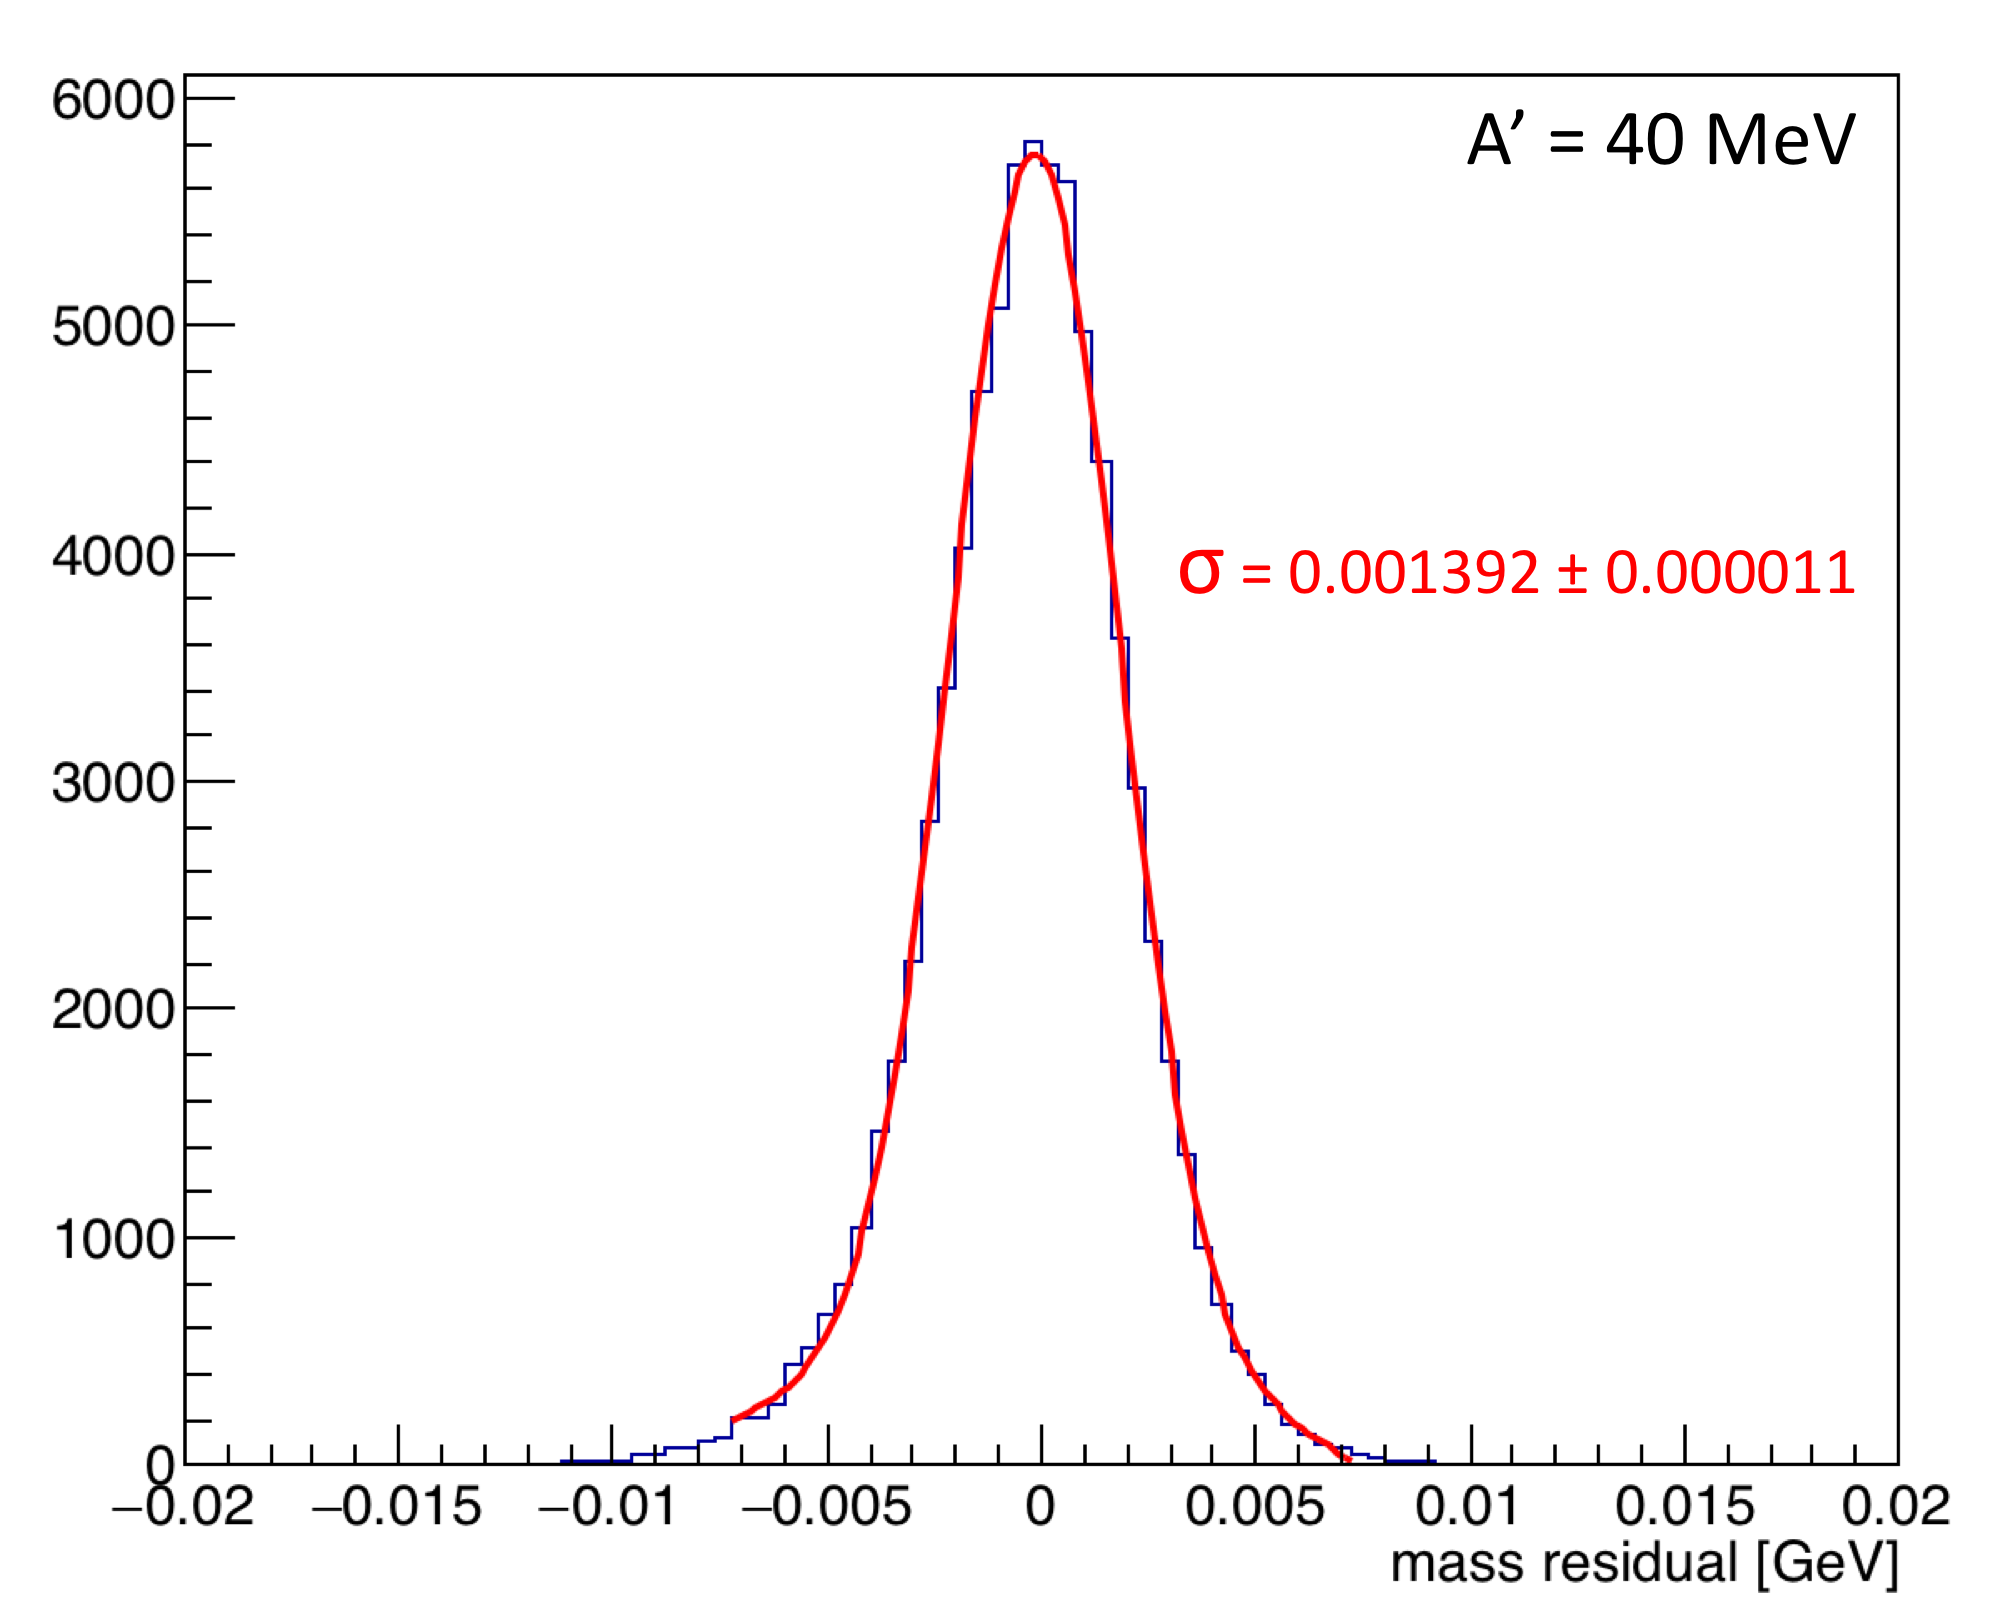
\includegraphics[width=0.5\textwidth]{pics/searching/ap40mev.png}
  \caption[Fit to the mass residual of a 40~MeV $A^{\prime}$]{The residual of a reconstructed 40~MeV $A^{\prime}$ mass is shown with a Gaussian fit.}
  \label{fig:ap40mev}
\end{figure} 

Simulations of the M\o ller mass can be used to study systematic offsets between the measured mass resolution in data and the mass resolution found in Monte Carlo. Using M\o ller Monte Carlo (with no beam background), the M\o ller mass can be seen on the left in Figure~\ref{fig:moller}. 

\begin{figure}[hbt]
%\begin{center}
\begin{minipage}{0.45\textwidth}
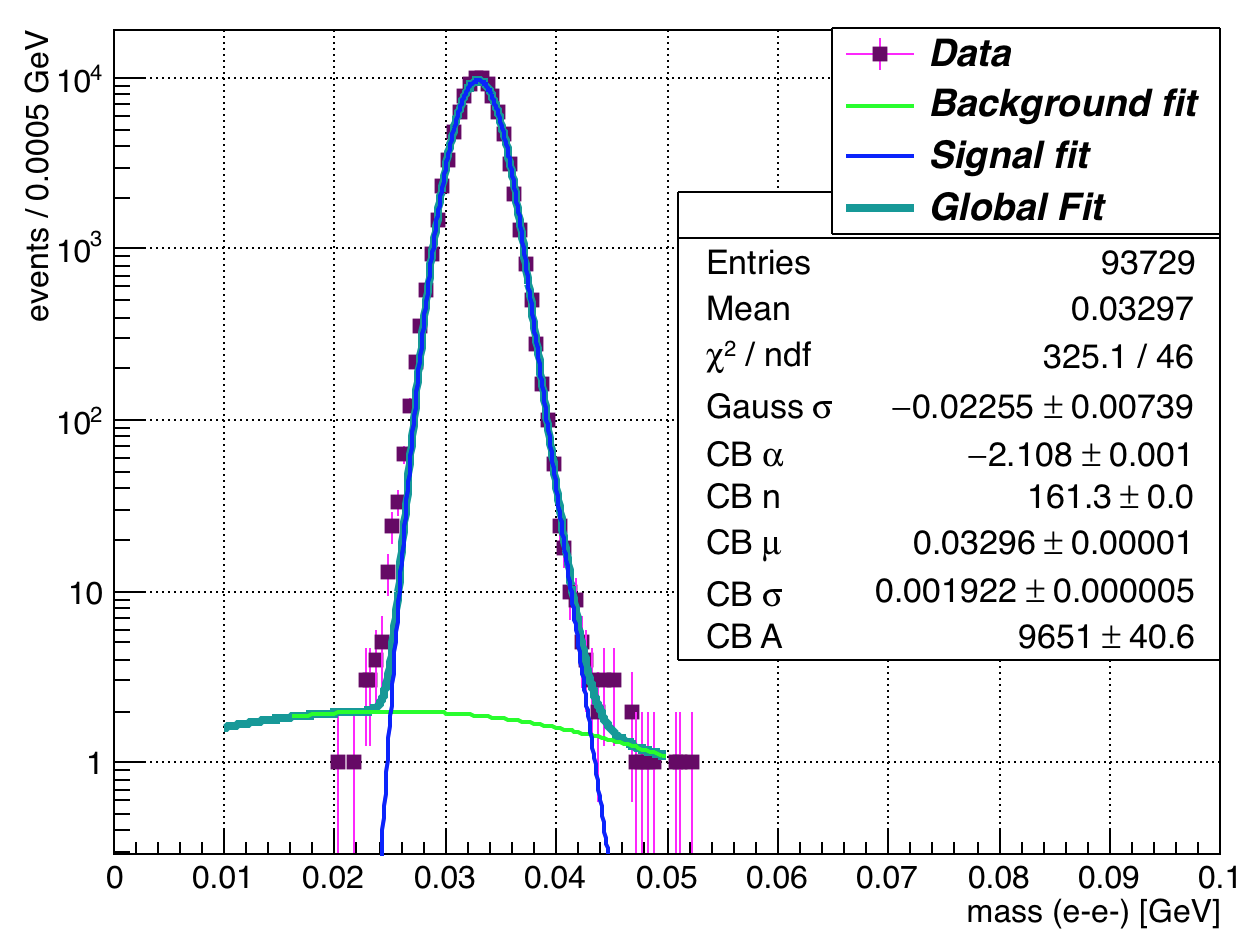
\includegraphics[width=\textwidth]{pics/searching/mollerMassMC.png}
%\end{center}
\end{minipage}\hfill\begin{minipage}{0.45\textwidth}
 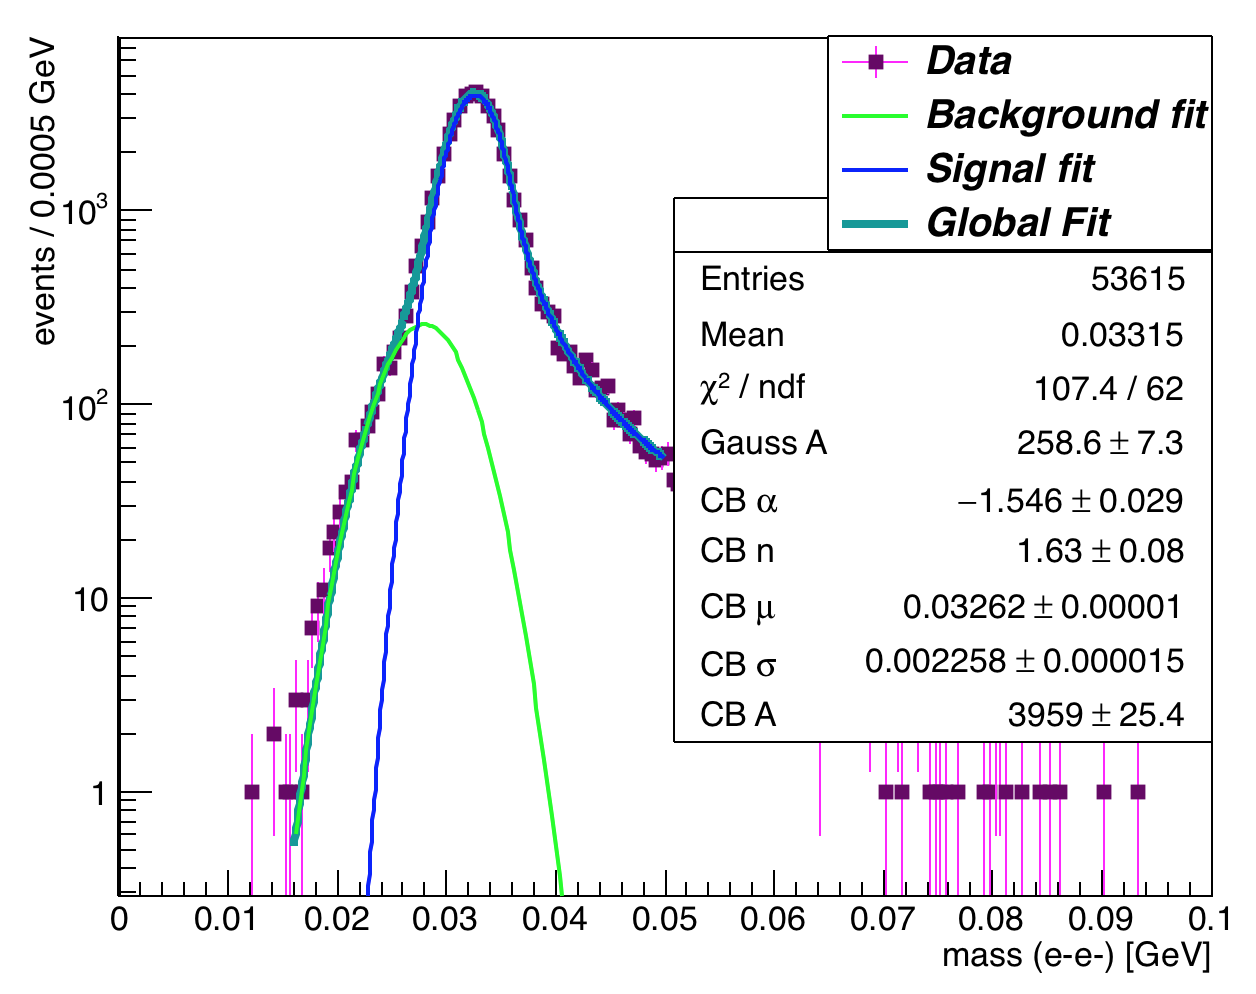
\includegraphics[width=\textwidth]{pics/searching/mollerMass.png}
 \end{minipage}
 \caption[Fit to the M\o ller mass peak in Monte Carlo and data]{The M\o ller mass peak from Monte Carlo with a Crystal Ball fit is shown on the left with the background fit using a Gaussian. The same fit models are then applied to the M\o ller mass in data, shown on the right.}
  \label{fig:moller}
\end{figure}
The M\o ller mass resolution from Monte Carlo is about 17$\%$ larger than the M\o ller mass resolution found in data. The heavy photon mass resolution found in Monte Carlo was increased by 17$\%$ in order to appropriately scale the bin widths when slicing and fitting the vertex distribution by mass. The M\o ller peak from data is shown on the right in Figure~\ref{fig:moller}. \\
\indent The mass resolution is shown in Figure~\ref{fig:massRes} as a function of mass. After applying the 17$\%$ scaling to the mass resolution from $A^{\prime}$ Monte Carlo, we obtain the mass resolution
\begin{equation}
\label{eq:massresScaled}
\sigma_m\textrm{[ GeV]} = 0.02436m+0.0007 \textrm{[ GeV]}
\end{equation}
used in the vertex analysis to find the $z$ vertex cut. 

\begin{figure}[hbt]
%\begin{center}
\begin{minipage}{0.65\textwidth}
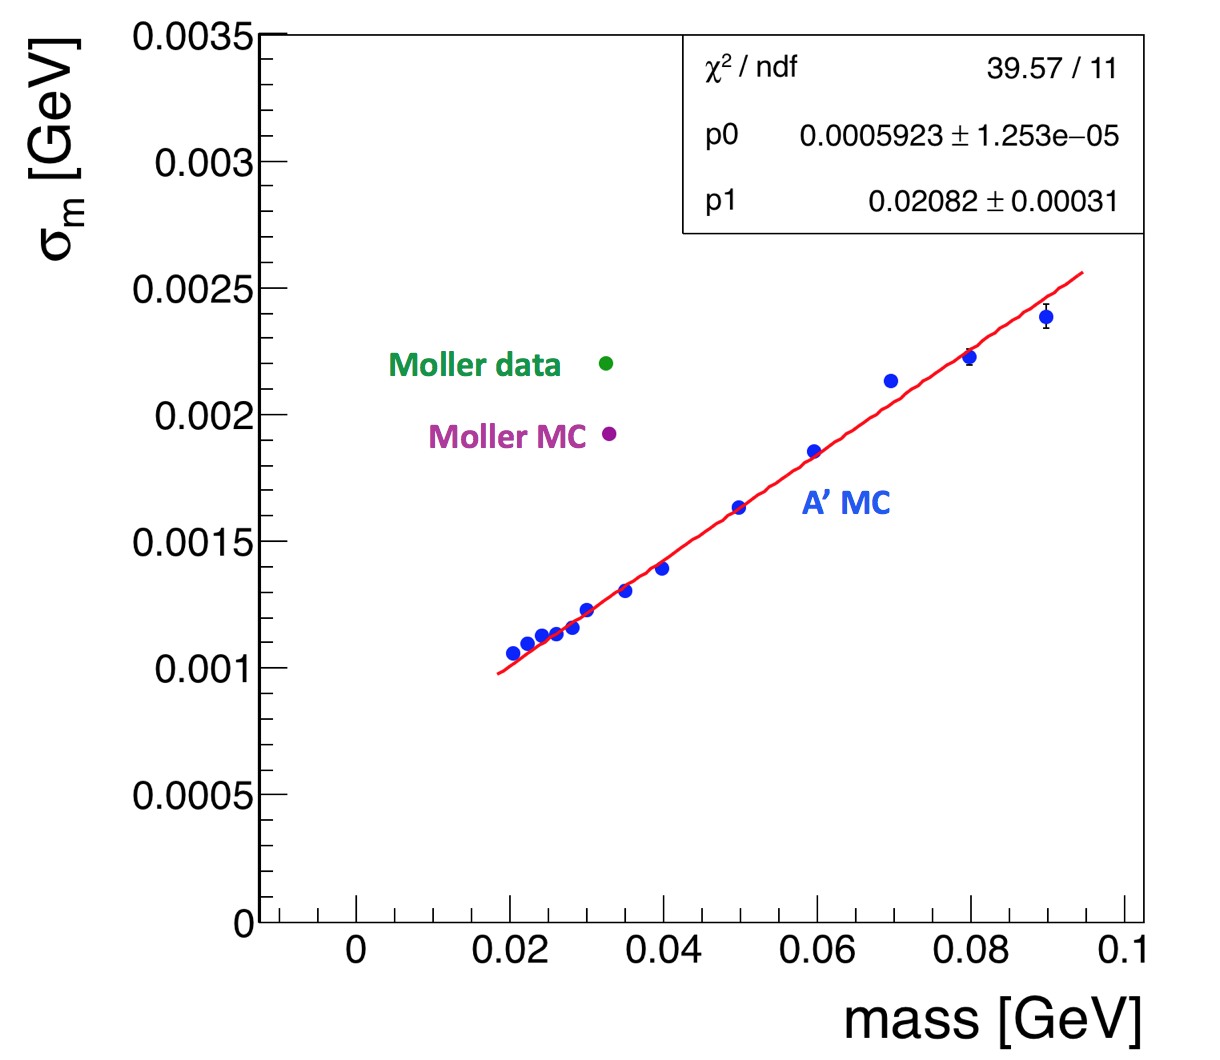
\includegraphics[width=\textwidth]{pics/searching/massResolution.png}
%\end{center}
\end{minipage}\hfill\begin{minipage}{0.32\textwidth}
\caption[Mass resolution compared between Monte Carlo and data]{ \label{fig:massRes} \baselineskip 11pt
The mass resolution for M\o ller data (green), M\o ller Monte Carlo (magenta), and $A^{\prime}$ Monte Carlo (blue) is shown. The red line $\sigma_m\textrm{[ GeV]} = 0.02082m+0.0006\textrm{[ GeV]}$ is fit to the $A^{\prime}$ mass resolution. The difference between the Monte Carlo and data M\o ller mass resolutions is approximately 17$\%$. This scaling should be applied to the linear fit of the $A^{\prime}$ mass resolution from Monte Carlo in order to account for the difference in resolution.
}
\end{minipage}
\end{figure}

%\section{Combining Ecal and SVT measurements}
%include a short discussion on this if time allows

\section{Vertex cuts}
The cuts used in the vertex analysis were generally derived from a study of 10$\%$ of the data and from Monte Carlo. In order to avoid a systematic bias, the 10$\%$ was selected from every tenth file. The following discussion will focus on the cuts used for the L1L1 0.5~mm data set. The effects of the cuts on the L1L2 and L2L2 data sets and the 1.5~mm data are discussed in Appendix~\ref{appendix:vtxCuts}. Improvements to cuts that were found after unblinding the full data set are discussed separately.\\ 

\subsection{Cuts tuned on 10$\%$ of the data}
Here, I will first summarize the cuts before discussing them in detail. The cuts used on the L1L1 0.5~mm data set are shown in Table~\ref{tab:l1l1_cuts}.

\begin{table}[htb]
\caption{Cuts applied to the L1L1 data set.}
\label{tab:l1l1_cuts}
\centering
\begin{tabular}{llllll}
\toprule
%\multicolumn{2}{c}{Name} \\
%\cmidrule(r){1-2}
Cut type & Cut & Cut Value &  $\%$cut &  $\%$cut core & $\%$cut tails\\
\midrule
track & Fit quality & track $\chi^{2}<30$ & 60 & 34 & 87 \\
track & Max track momentum &  $P_{trk}<75\%E_{beam}$ & 11 & 9 & 22 \\
track & Isolation &   & 4 & 2 & 19 \\
vertex & beamspot constraint & bsc$\chi^{2}<10$  & 26 & 20 & 72 \\
vertex & beamspot - unconstrained & bsc$\chi^{2}$-unc$\chi^2<5$  & 9 & 9 & 21 \\
vertex & maximum $P_{sum}$ &  $<115\%E_{beam}$ & 1 & 0 & 2 \\
ecal & Ecal SVT matching & $\chi^2<10$  & 7 & 6 & 49 \\
ecal & track Ecal timing & $<4$ns  & 4 & 4 & 7 \\
ecal & 2 cluster time diff & $<2$ns  & 6 & 6 & 13 \\
physics & momentum asymmetry & $<0.4$  & 13 & 13 & 27 \\
physics & e+ track d0 & $<1.5$mm  & 0 & 0 & 1 \\
event & max shared hits amongst tracks & $<5$ shared hits  & 14 & 14 & 15 \\
\bottomrule
\end{tabular}
\end{table}


In Table~\ref{tab:l1l1_cuts}, the ``Cut type" is a summary of what the cut is intended to have the most significant effect on. The ``Cut" describes the cut used, and the corresponding value is shown in the next column, ``Cut Value". The ``$\%$ cut" column shows the percentage of the  events removed from the entire data set by applying this cut. The ``$\%$ cut core" column shows the percentage of events removed from the Gaussian core of the vertex distribution. The ``$\%$ cut tails" column shows the percentage of events removed from the downstream tails of the vertex distribution. Our cuts aim to remove background events in the downstream vertex tails.\\
\indent The effects of the cuts on the $z$ vertex for all masses is shown in Figure~\ref{fig:l1l1_vtx} in the cumulative order in which the cuts are applied. The initial track fit $\chi^{2}$ from the GBL fit of the track removes a lot of background and begins to really shape the vertex distribution. The next significant cut is the beamspot constrained $\chi^{2}$ cut. The beamspot constrained $\chi^{2}$ includes both the closest approach of the two tracks and the momentum projection of the vertex back to the beamspot position at the target. The momentum asymmetry is a cut that is primarily designed to remove WAB contributions to the data. Heavy photon generated $e^+e^-$ pairs are generally close in energy whereas the electron in WAB typically carries a much larger energy than the counterpart photon.\\ 
\indent The last cut listed in Table~\ref{tab:l1l1_cuts} removed events where either of the $e^+e^-$ individual tracks shared five hits with other tracks. When studying the original high $z$ background, nearly all of the high $z$ events were poorly reconstructed tracks due to missing hits in Layer 2 or to sharing five hits with other tracks in the event having nearly the same momentum. The cuts cleaned up the high $z$ background in the 10$\%$ data set. The effects of the cuts on the $z$ vertex distribution can be seen in Figure~\ref{fig:l1l1_vtx}.

\begin{figure}[hbt]
%\begin{center}
\begin{minipage}{0.5\textwidth}
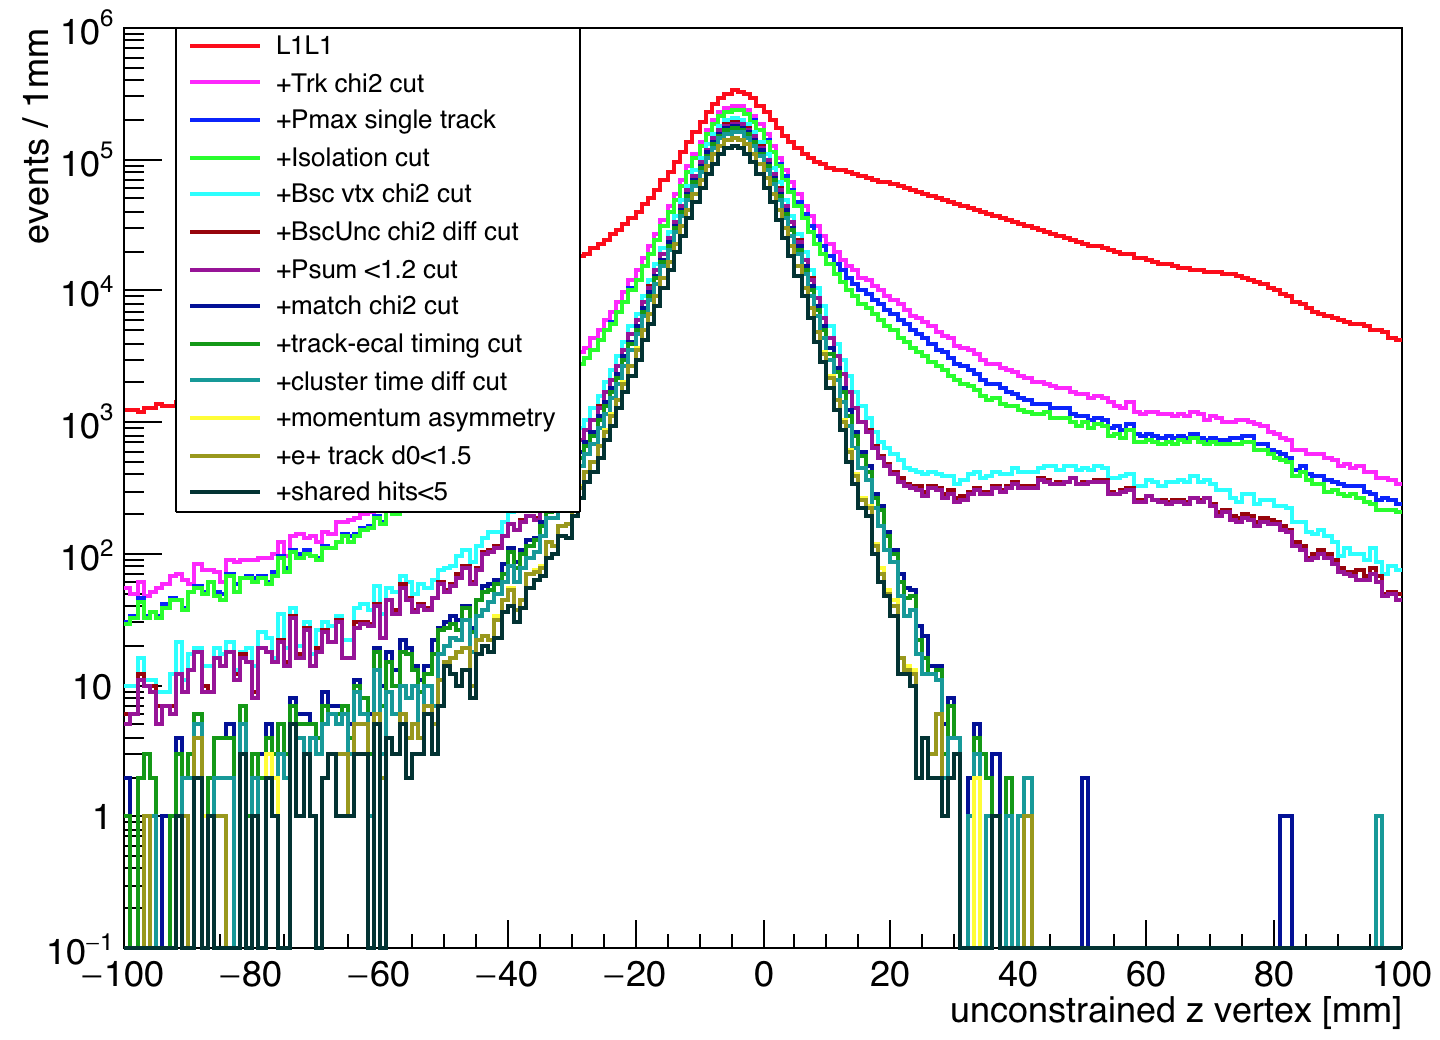
\includegraphics[width=\textwidth]{pics/searching/L1L1_zvtx.png}
%\end{center}
\end{minipage}\hfill\begin{minipage}{0.5\textwidth}
 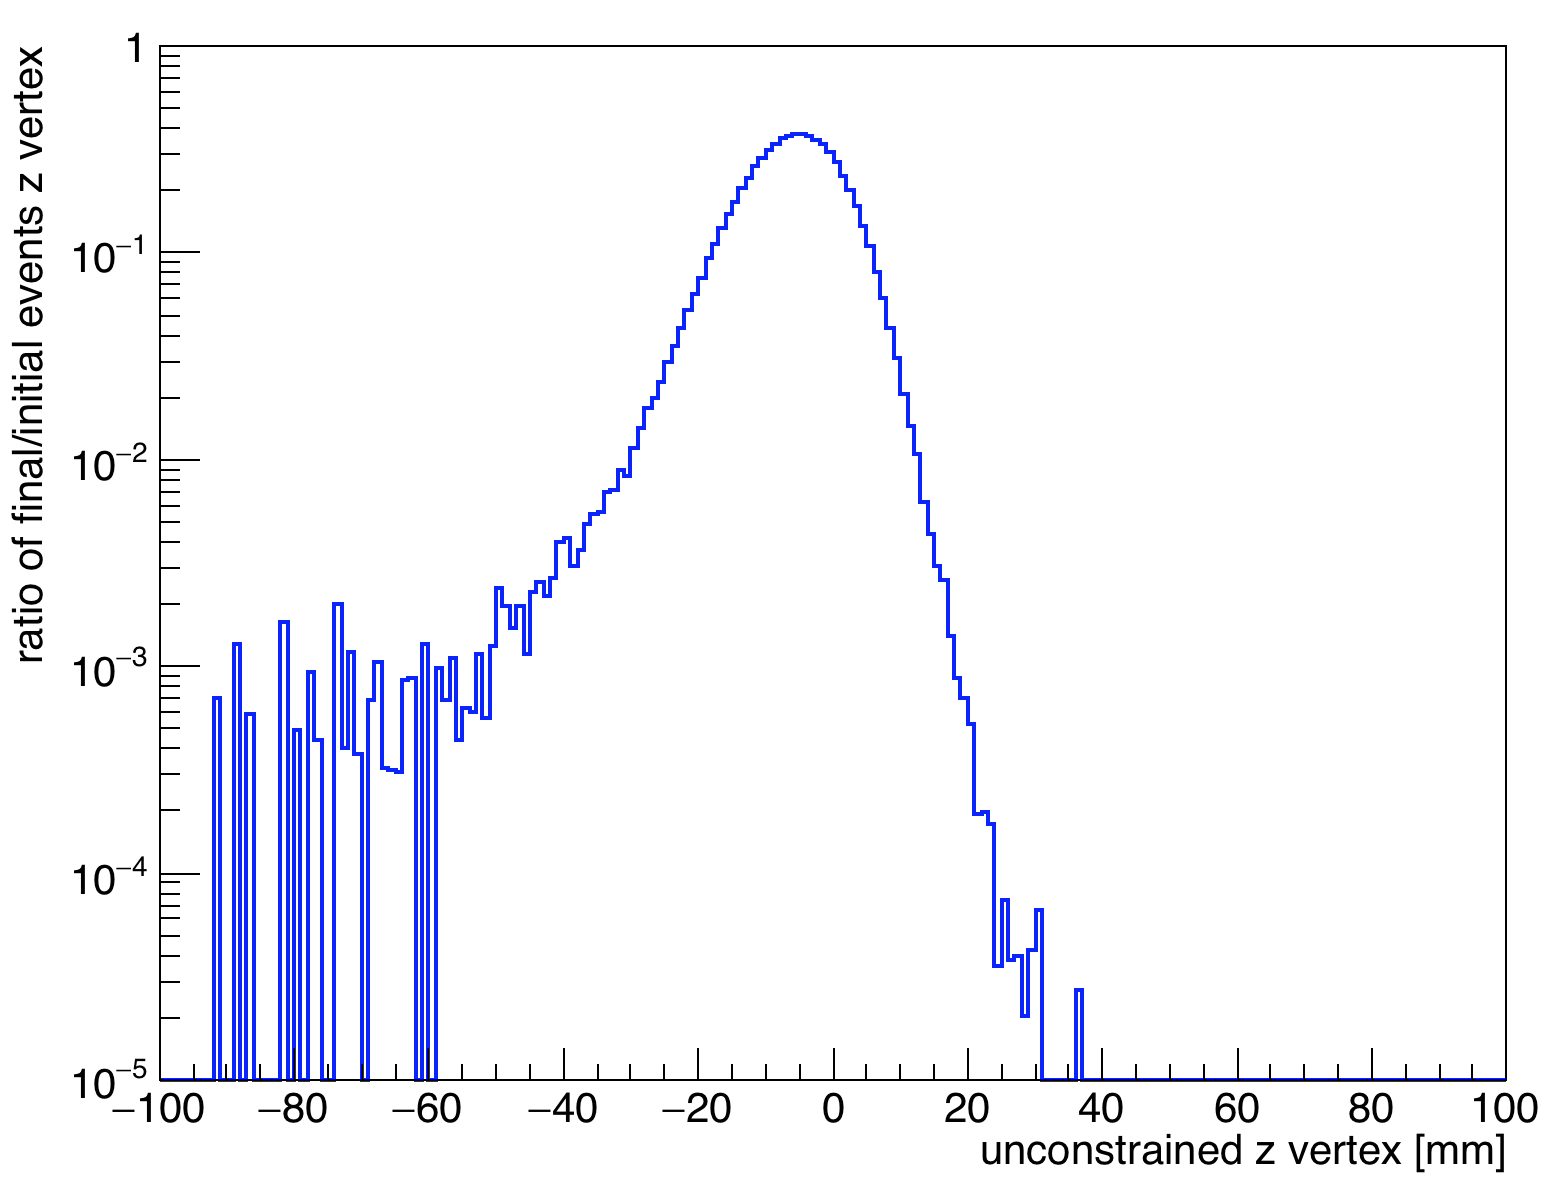
\includegraphics[width=\textwidth]{pics/searching/ratio_zvtx_cuts.png}
 \end{minipage}
 \caption[Cut effects on the $z$ vertex distribution]{Cut effects on the $z$ vertex distribution for all masses in the L1L1 0.5~mm dataset is shown on the left.The ratio of the $z$ vertex distribution in the final event selection to those events in the initial event selection in the L1L1 0.5~mm dataset is shown on the right.}
  \label{fig:l1l1_vtx}
\end{figure}
The two cluster time difference can be used to study the effects of cuts on accidentals as well as the contamination of accidentals in the final sample. The evenly spaced 2~ns peaks as apparent in Figure~\ref{fig:l1l1_tdiff} are due to the intrinsic 499~MHz electron beam bunch frequency.

\begin{figure}[hbt]
%\begin{center}
\begin{minipage}{0.45\textwidth}
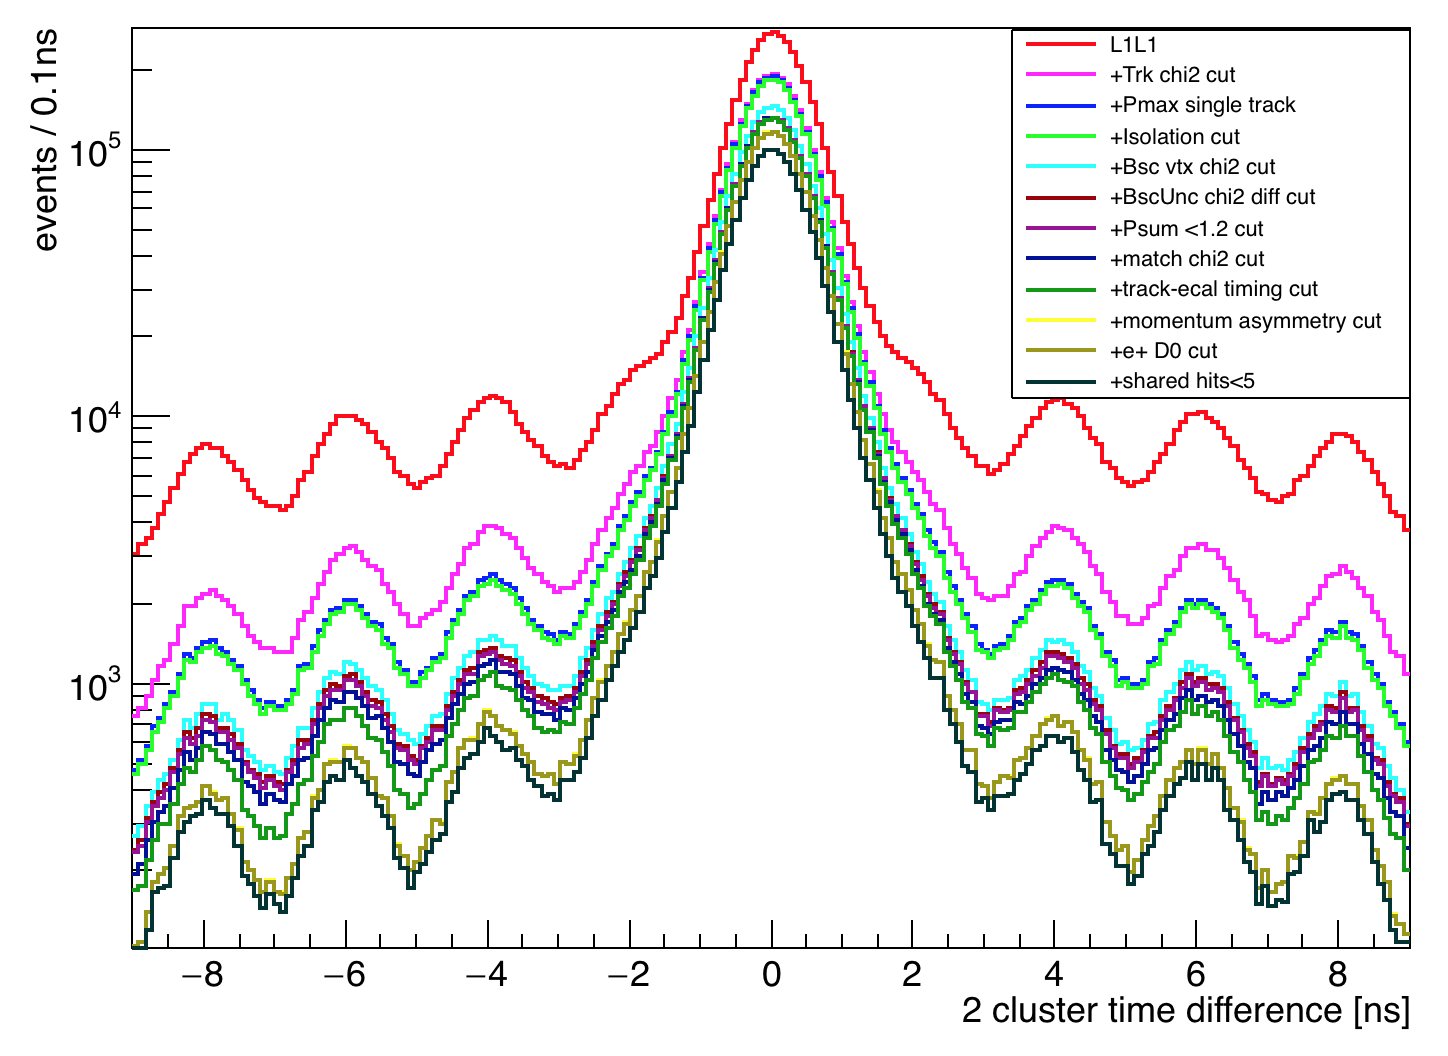
\includegraphics[width=\textwidth]{pics/searching/L1L1_tdiff.png}
%\end{center}
\end{minipage}\hfill\begin{minipage}{0.45\textwidth}
 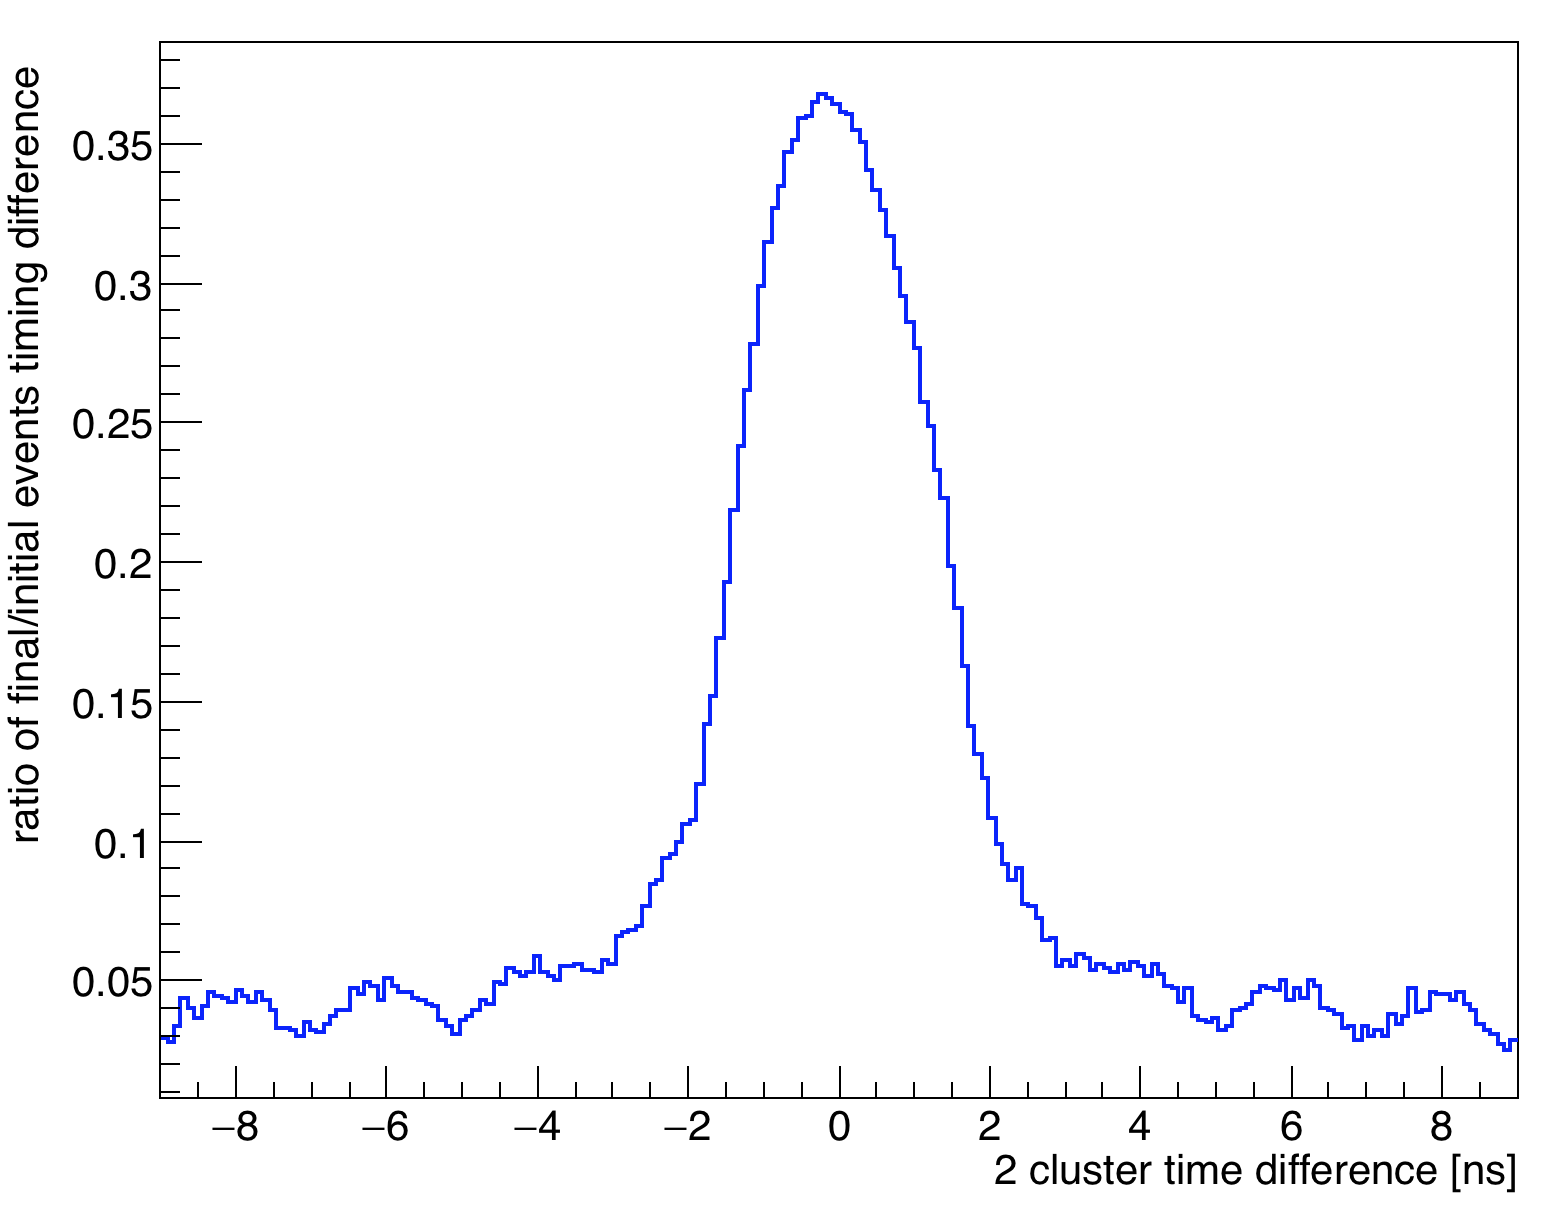
\includegraphics[width=\textwidth]{pics/searching/ratio_tdiff_cuts.png}
 \end{minipage}
 \caption[Cut effects on the time difference between two clusters]{Cut effects on the two cluster time difference distribution for the L1L1 0.5~mm dataset is shown on the left.The ratio of the two cluster time difference distribution in the final event selection (without the $\pm2$~ns cut) to those events in the initial event selection for the L1L1 0.5~mm dataset is shown on the right.}
  \label{fig:l1l1_tdiff}
\end{figure}

After all cuts are applied, the accidental contamination is less than 1$\%$ in the $\pm$ 2~ns event selection (this cut is the only one not shown in Figure~\ref{fig:l1l1_tdiff}). Further studies to identify the production of events with high $z$ vertices using accidentals is discussed later on in this section. The cut effects on the mass distribution for the vertex search can be seen in Figure~\ref{fig:l1l1_mass}. In particular, the track-cluster matching removes the low mass tail of the mass distribution which is consistent with the geometric acceptance of the experimental setup.

\begin{figure}[htb]
  \centering
      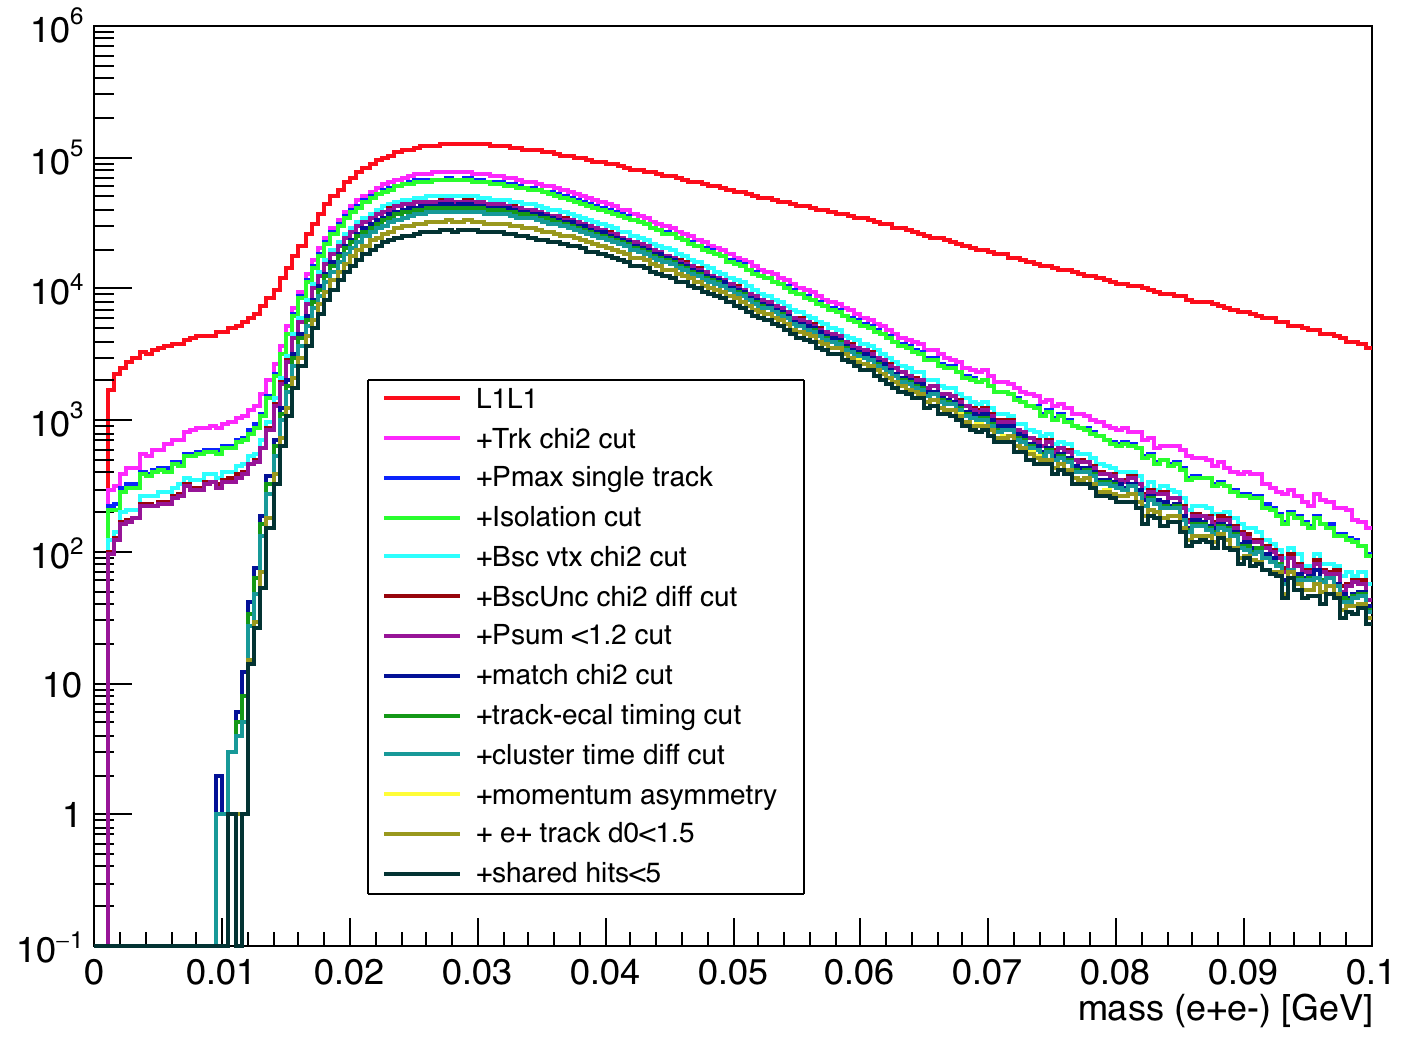
\includegraphics[width=0.75\textwidth]{pics/searching/mass_L1L1_cuts.png}
  \caption[Cut effects on the mass distribution]{Cut effects on the mass distribution for the L1L1 0.5~mm dataset.}
  \label{fig:l1l1_mass}
\end{figure} 

\begin{figure}[htb]
  \centering
      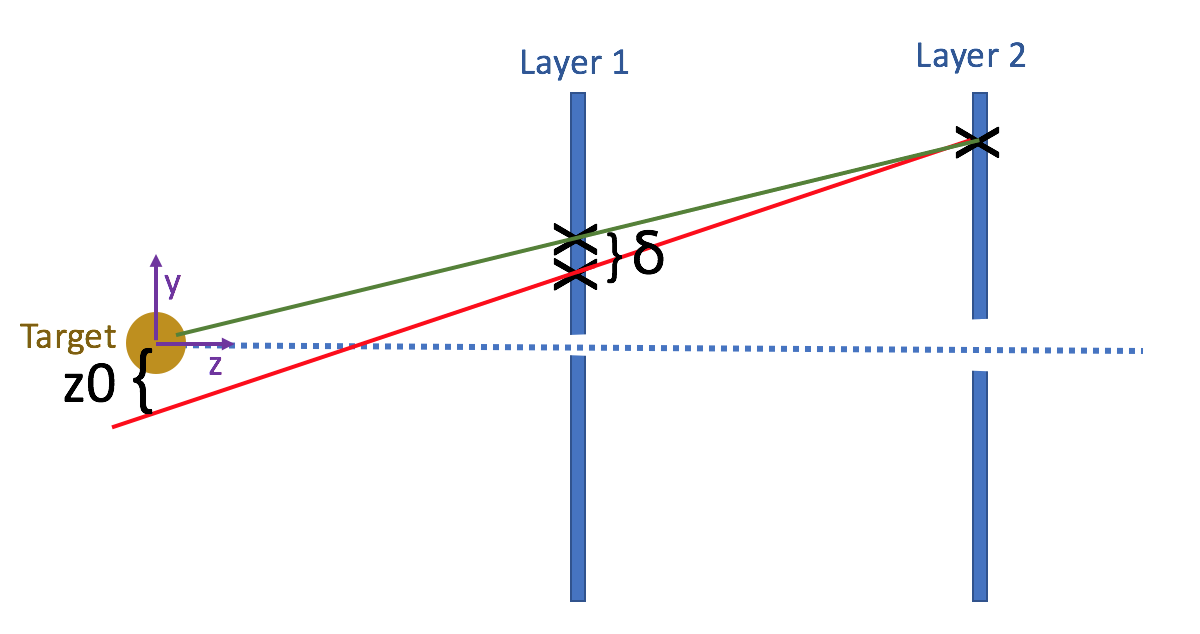
\includegraphics[width=0.6\textwidth]{pics/searching/isolationPic.png}
  \caption[Track isolation cut]{The distance between the closest hit away from the beam in Layer 1 is compared to its projection at the target, the track impact parameter $z0$. }
  \label{fig:isoPic}
\end{figure}
The L1L1 dataset requires that both tracks have hits in both Layers 1 and 2 of the SVT. Previously, the requirement of Layer 2 was not used, but as the rates are highest in Layer 1 of the SVT, the extrapolation from Layer 3 to Layer 1 is critical in order to correctly measure the vertex of the track. Additionally, the inefficiency in measuring a hit in Layer 2 is approximately 2$\%$ (and is different for electrons and positrons). Included in the initial event selection is also the radiative cut at 80$\%$ of the beam energy. After these initial cuts, we apply the track selection cuts. To ensure general track quality, the track $\chi^2$ is cut at $\chi^2<30$ for both the electron and positron tracks as shown in Figure~\ref{fig:trkChi2} in Appendix~\ref{appendix:vtxCuts}.\\
\indent After choosing tracks based on their individual fit qualities, we remove electron tracks that have greater than 75$\%$ of the beam energy. This cut is made to ensure that we are not choosing elastically-scattered (beam energy) electrons and corresponds also to the general maximum value we can expect for an electron track in trident events. A comparison between the data and Monte Carlo is shown in Figure~\ref{fig:emTrkPmax} in Appendix~\ref{appendix:vtxCuts}. \\
\indent The next cut applied is the isolation cut. The isolation value for the electron and the positron in the L1L1 dataset is the distance to the next closest hit away from the beamline in Layer 1 relative to the electron and positron hit used in the track. This cut compares the isolation value (parameter $\delta$) to the track projected value in $y$ at the target position (also known as the track $z0$ parameter). If the projected isolation to the target is larger than the $z0$ parameter at the target, then we assume that the better hit was already chosen for the track. A picture of the variables used in this cut is shown in Figure~\ref{fig:isoPic} and described numerically in Equation~\eqref{eq:isolationl1}.

\begin{equation}
\label{eq:isolationl1}
2\delta+z0\times\textrm{sign($P_y$)}>0
\end{equation}
The factor of 2 comes from the ratio of the distance from Layer 2 to the target and the distance from Layer 1 and the target. The $z0$ parameter is opposite in sign as compared to the $y$-component of the track momentum because we only consider downstream vertices. \\
\indent In identifying downstream vertices, we use the unconstrained vertex collection to optimize our search for detached vertices. For each vertexed $e^+e^-$ pair, we can see how the vertex changes when different additional constraints are applied. The unconstrained vertex collection only looks at the distance of closest approach between the two tracks. The target constrained vertex collection is optimized for a bump hunt analysis and requires that the vertex of the $e^+e^-$ pairs occurs at the target. The beamspot constrained vertex collection requires that the momentum of the vertexed pairs projects back to the beamspot location at the target and considers the distance of closest approach between the two tracks.\\ 
\indent The beamspot constrained vertex fit quality, or vertex $\chi^2$, gives us information about how well the vertex momentum points back to the beamspot location at the target. The beamspot constraint is particularly useful in identifying events where a track has scattered significantly because the the projected momentum misses the beamspot location at the target. Real signal events will always project back to the beamspot. The effect of the beamspot constraint cut on the vertex  $\chi^2$ distribution alone can be seen in Figure~\ref{fig:bsccut}.

\begin{figure}[htb]
  \centering
      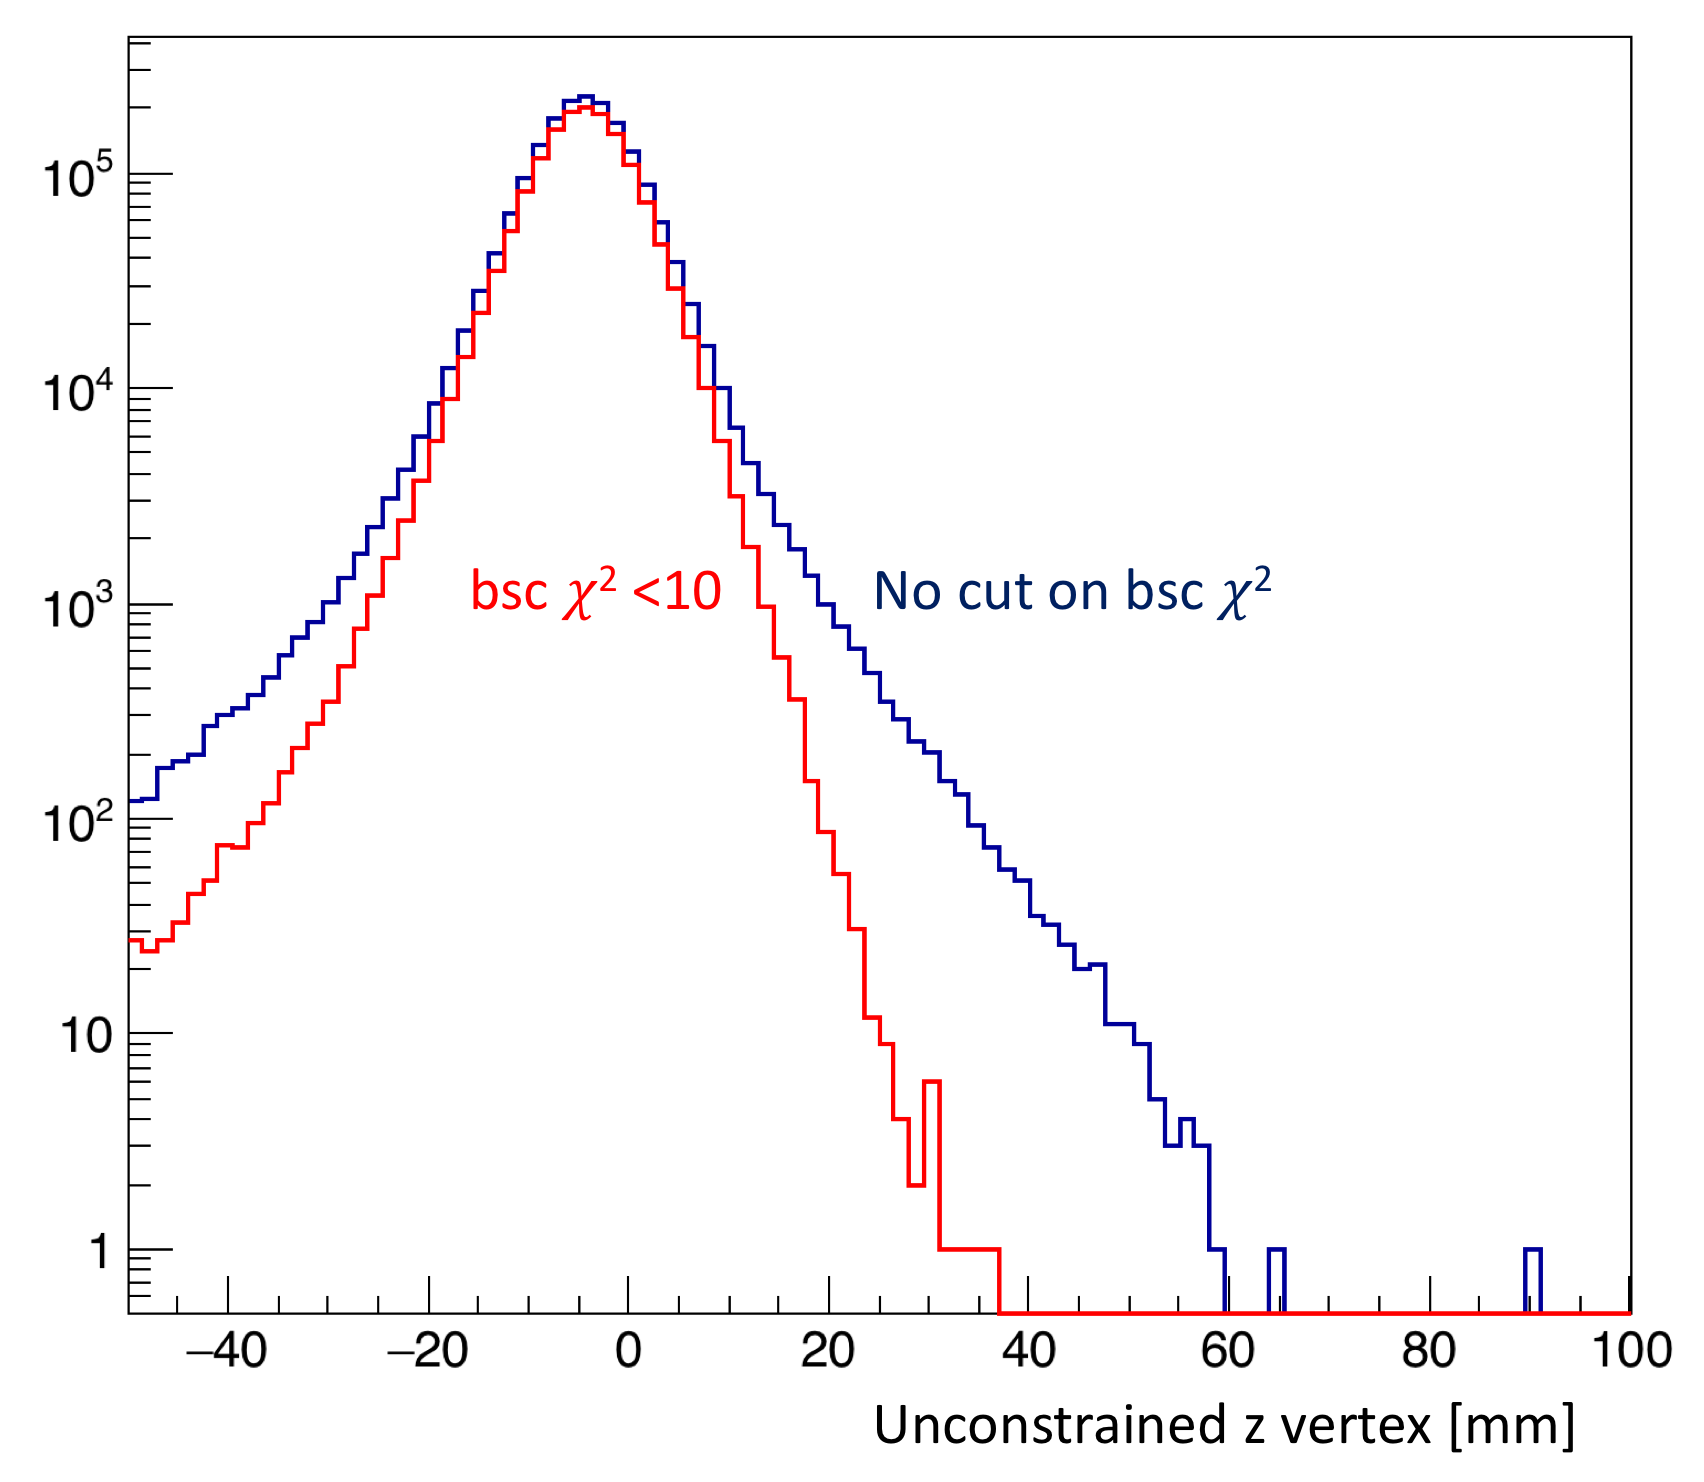
\includegraphics[width=0.6\textwidth]{pics/searching/bscCut.png}
  \caption[Cut on beam spot constrained vertex $\chi^2$]{The effect of a cut on the beamspot constrained $\chi^2$ on the vertex distribution for all masses. While this plot is shown for all masses, the effects of the cut on the tails of the distribution can still be seen. The cut removes events where tracks did not pass close to each other in space to generate a vertex and/or the vertex does not point back to the beam position at the target.}
  \label{fig:bsccut}
\end{figure} 

The difference between the beamspot constrained and unconstrained $\chi^2$ can also be used to exclusively identify how well a vertex points back to the target. The effect of this cut can be seen in Figure~\ref{fig:bmucut} in Appendix~\ref{appendix:vtxCuts}.\\
\indent The next cut is the maximum momentum of the $e^+e^-$ pair. This cut removes very few events but is still necessary to ensure that we are not including events that are not correlated. \\
\indent After having established the quality of the tracks and vertex using the SVT information only, the tracks are projected to their positions at the ECal and the quality of the matching of the track and ECal cluster is described as a multiple of the expected resolution function of the track momentum and position at the ECal. This parameter is a function of the number of $\sigma$ from distributions studied used 2015 data. The matching parameter and relevant cut value are shown in Figure~\ref{fig:matchcut} in Appendix~\ref{appendix:vtxCuts}. \\
\indent The matching cut most significantly removes the small angle/low mass background events that we saw in Figure~\ref{fig:l1l1_mass}. The timing difference between the tracks and ECal clusters removes some out of time events, but the timing resolution on the clusters is more precise than the track time and a cut on the two cluster time difference is critical for removing accidentals. The cut on the cluster time difference is shown in Figure~\ref{fig:cltdiff} in Appendix~\ref{appendix:vtxCuts}.\\
\indent Additional cuts aimed to remove the wide angle breamsstrahlung background events include a cut on the momentum asymmetry of the two tracks and the positron $D0$, or $DOCA$ (distance of closest approach to the target in the $x-z$ plane), are used. The momentum asymmetry is defined as the momentum difference of the two particles divided by the momentum sum. The $e^+e^-$ pairs produced in radiative trident processes from heavy photon decays have similar momentum. The electron in wide-angle bremsstrahlung typically carries a significantly higher fraction of the beam energy than the positron that is produced from the pair production of the lower energy photon. The effect of the momentum asymmetry cut on the vertex distribution is shown in Figure~\ref{fig:pasycut} in Appendix~\ref{appendix:vtxCuts}.\\
\indent The momentum asymmetry cut can effectively reduce contamination from wide-angle bremsstrahlung in the final event sample. In wide-angle bremsstrahlung, the scattered electron and the positron from pair conversion are detected. When a positron is produced downstream of the target in this process, the projected $DOCA$ of the resultant track to the target will be positive due to the curvature of the positron track in the magnetic field from starting downstream. The cut on the $DOCA$ is shown in Figure~\ref{fig:docacut}. 

\begin{figure}[htb]
  \centering
      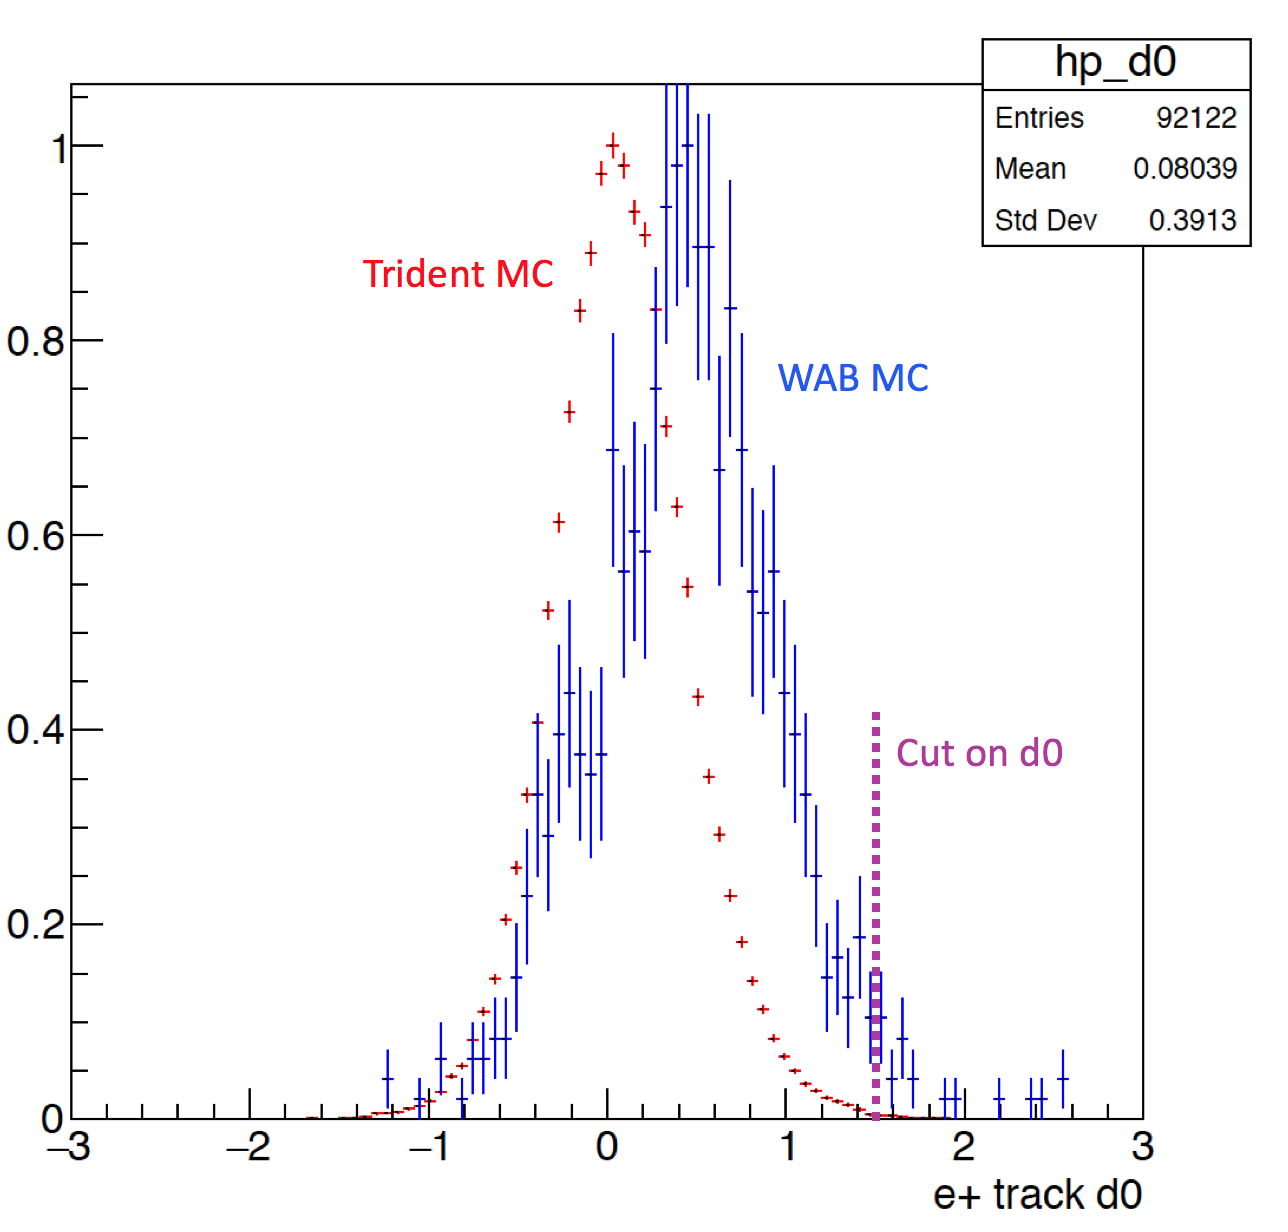
\includegraphics[width=0.6\textwidth]{pics/searching/epd0cut.png}
  \caption[Cut on the $e^+$ $DOCA$ to remove WAB]{Positrons that are produced downstream of the target from pair production of the photon in WAB have a positive $DOCA$. The tridents have a symmetric distribution about 0. The cut value is indicated by the dashed purple line. The effects of this cut on the vertex distribution are shown in the Appendix~\ref{appendix:vtxCuts}.}
  \label{fig:docacut}
\end{figure} 

The final cut on tracks was derived after studies of the high $z$ background events showed a higher probability of one or both of the tracks sharing five hits with another track in the event. In these cases, the track with the best $\chi^2$ track fit is selected, but the momentum difference with the other track with which it shares five hits is quite small. The momentum difference of the track with the other tracks that share hits is shown versus the number of hits shared between the tracks in Figure~\ref{fig:trkshare}  in Appendix~\ref{appendix:vtxCuts}. By removing tracks that only have a one hit difference with other tracks, the high $z$ background in the data sample is reduced.   

%\subsection{Additional cuts}%Wednesday
%Discuss the additional cuts after unblinding: matching, track chi2/dof, kink cuts
\section{Initial selection of the 10$\%$ sample}
After applying all of the previously discussed cuts as tuned on the 10$\%$ data sample, we see the resulting $z$ vertex distribution as a function of corrected mass in Figure~\ref{fig:zVm_bl}.

\begin{figure}[htb]
  \centering
      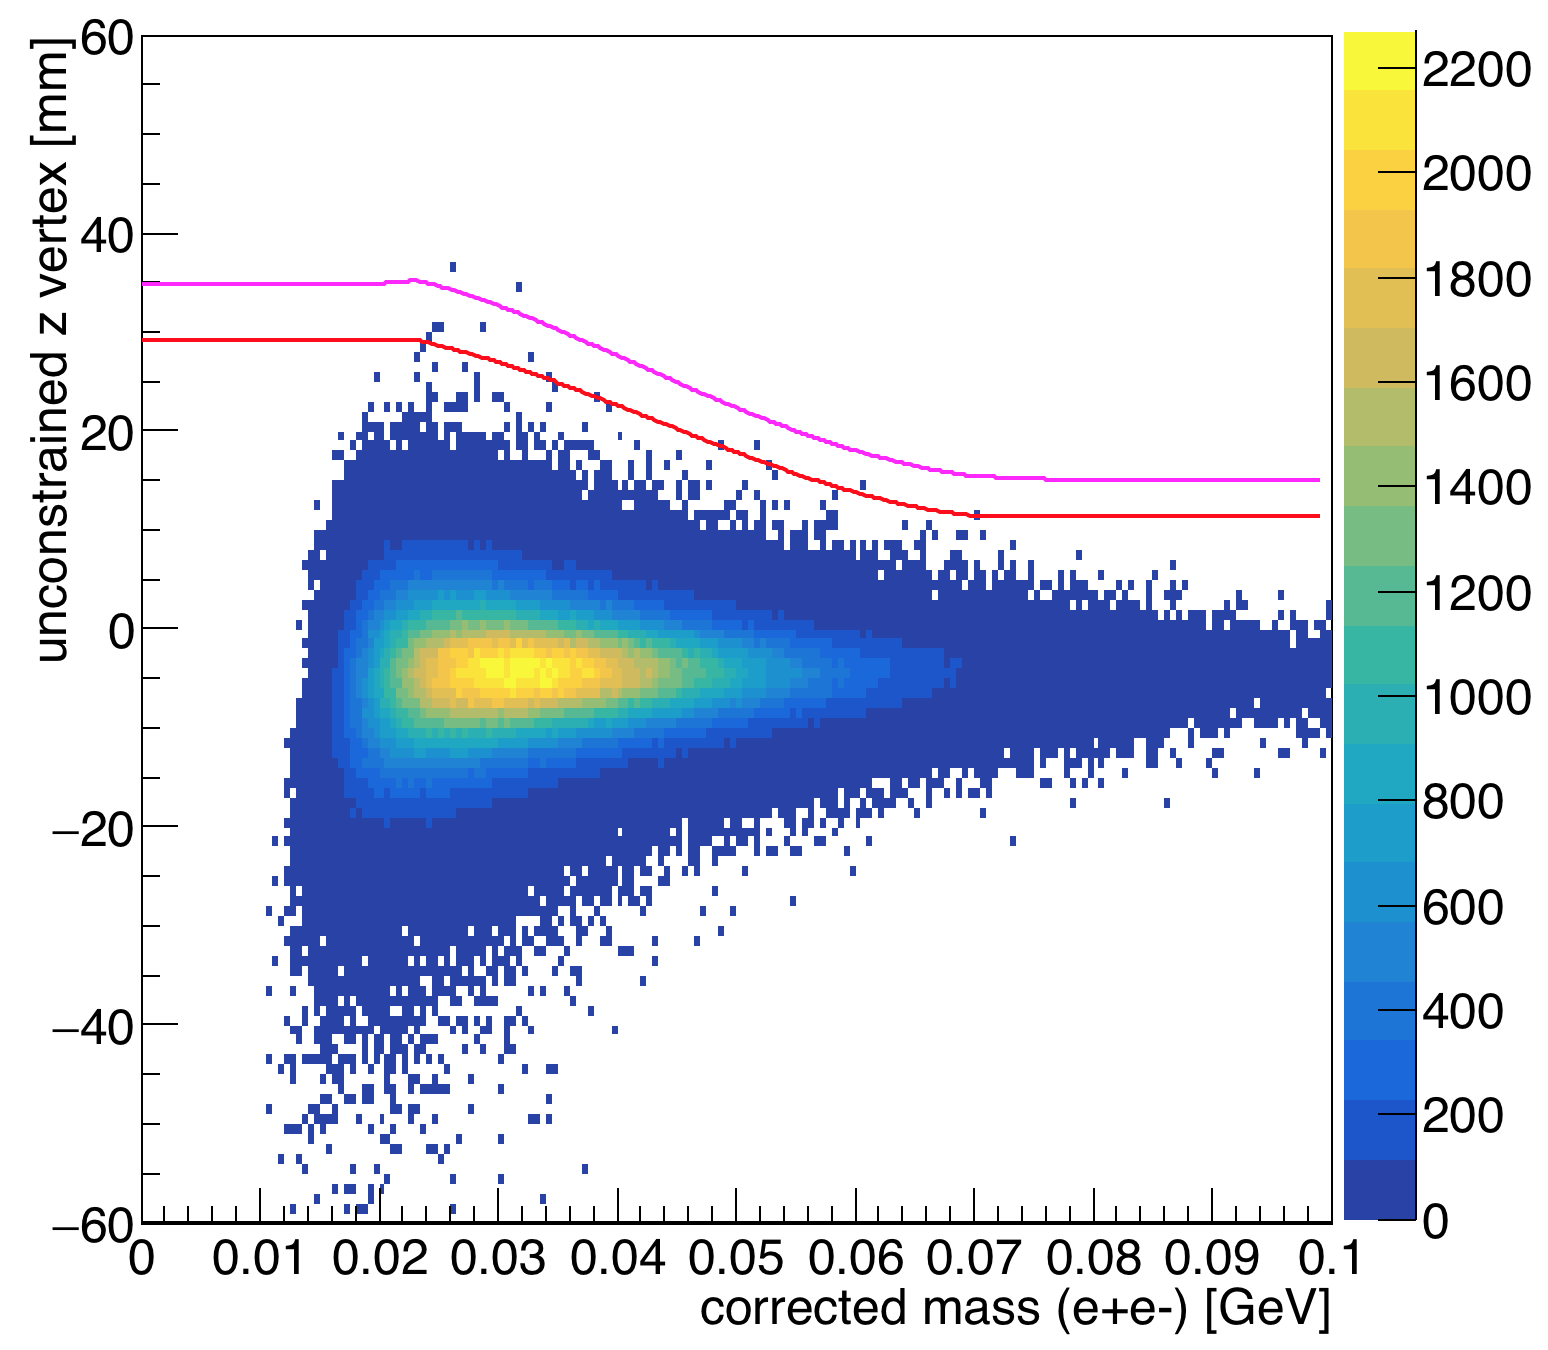
\includegraphics[width=0.75\textwidth]{pics/searching/zVm_bl_L1L1.png}
  \caption[Vertex position vs mass for the 10$\%$ L1L1 data]{The unconstrained $z$ vertex position is shown as a function of the corrected mass of the $e^+e^-$ pair. The $zCut$ as measured for this data is shown in red and corresponds to where there is less than 0.5 background event beyond. The projected $zCut$ for the full 100$\%$ data is shown in magenta. The relevant mass range used to fit $zCut$ is from 0.02--0.07~GeV based on measured statistics.}
  \label{fig:zVm_bl}
\end{figure} 

From this initial sample, we still see that there are 3 events in the high $z$ region that will be apparent in the full 100$\%$ dataset. In order to get a rough estimate from the contamination due to accidentals, vertices with cluster time differences greater than 3~ns and less than 9~ns were selected and the vertex distribution was studied. This time window was selected because SVT efficiency deteriorates outside of this and results in less reconstructed events. The accidental vertex distribution is shown in Figure~\ref{fig:zVm_acc}.

\begin{figure}[htb]
  \centering
      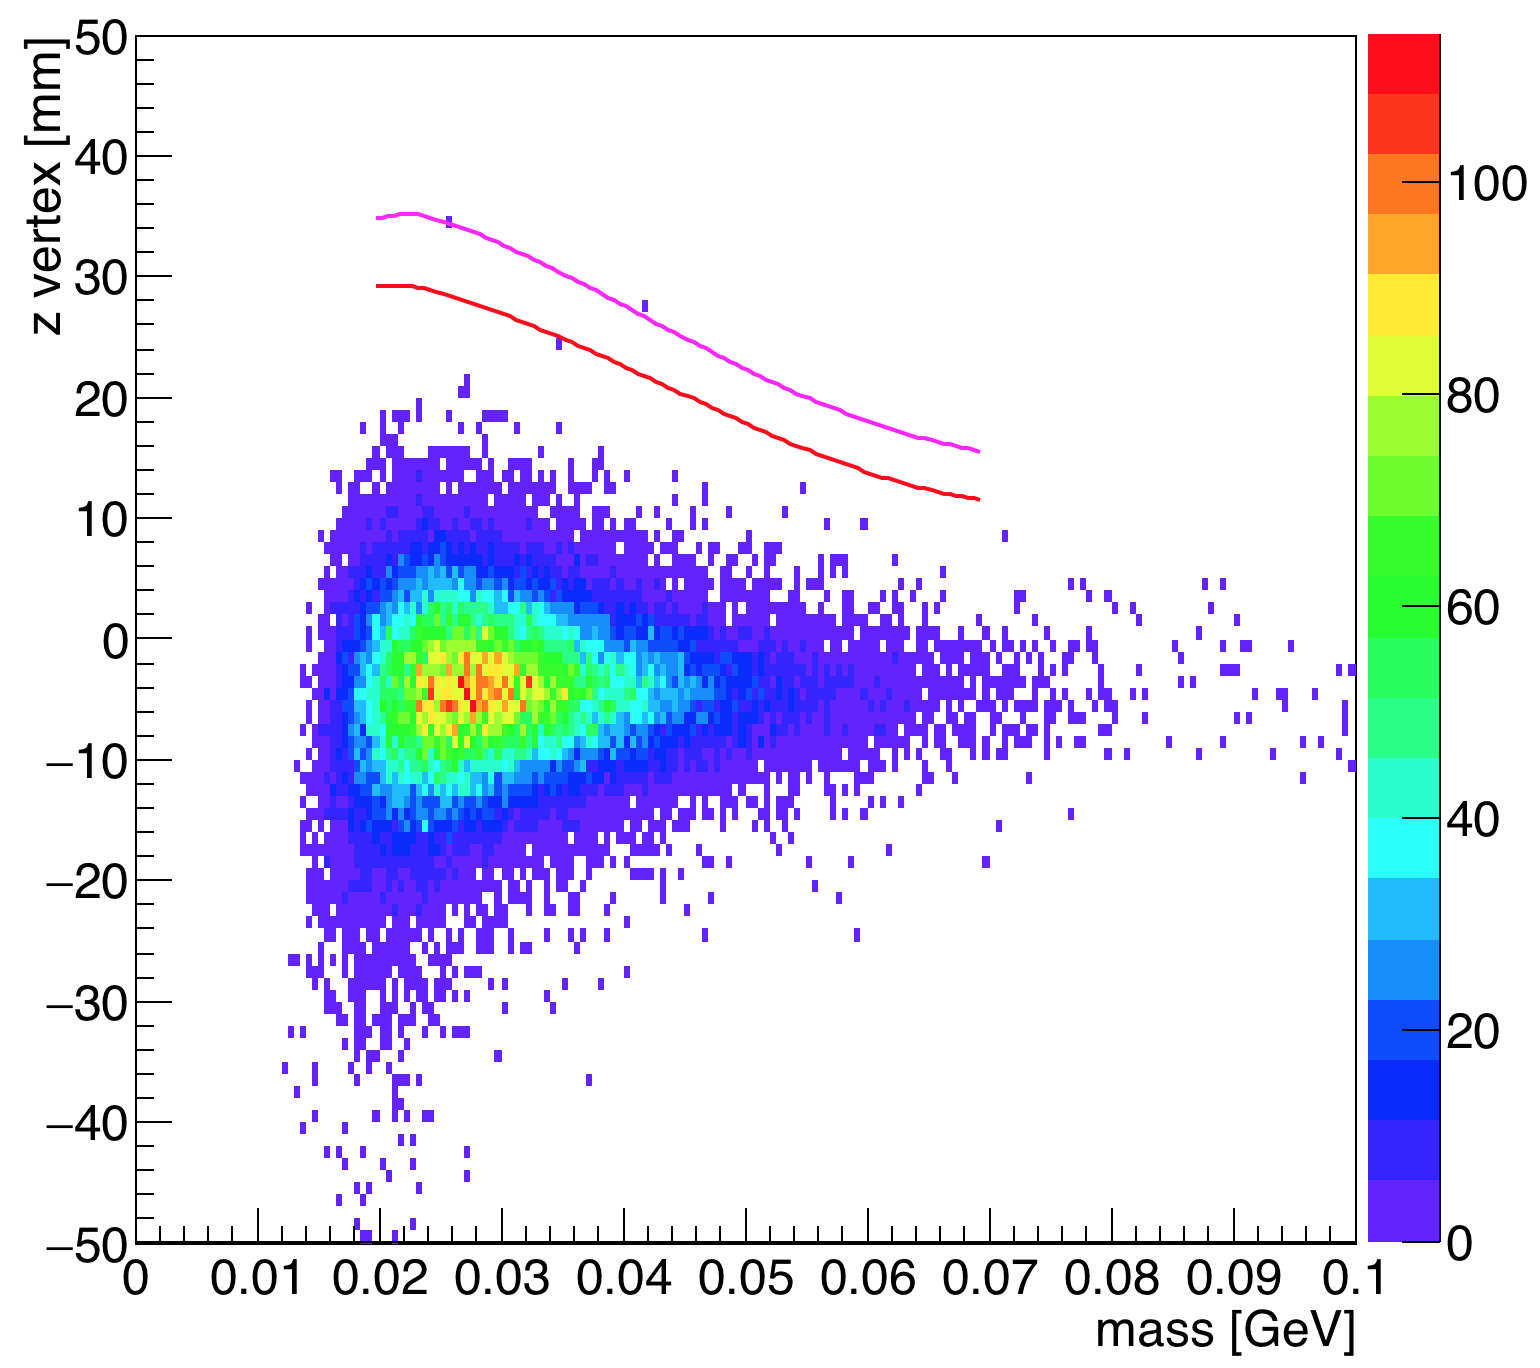
\includegraphics[width=0.75\textwidth]{pics/searching/zVm_acc_L1L1.png}
  \caption[Vertex position vs mass for the 10$\%$ L1L1 accidentals]{The unconstrained $z$ vertex position is shown as a function of the corrected mass of the $e^+e^-$ pair for out of time clusters. These events are selected such that the cluster time difference is greater than 3~ns and less than 9~ns covering a total of six beam buckets. There are three events that contaminate the high $z$ region from accidentals over the six beam buckets. The actual data selection uses clusters from two beam buckets.}
  \label{fig:zVm_acc}
\end{figure} 

In the accidental vertex distribution, we obtained 3 high $z$ events from the selected six beam buckets. The vertex events selected for the vertex search are centered on 2 beam buckets. Therefore, in the 10$\%$ sample, we may have $1\pm0.6$ high $z$ events attributable to accidentals. A rigorous procedure to identify the accidental rate would be to determine the vertex distribution of the electron selected from one event and the positron selected from another. One would expect the effects from the high $z$ background to scale by a factor of 10 to the final full data set. 